\documentclass[conference]{IEEEtran}
\IEEEoverridecommandlockouts
% The preceding line is only needed to identify funding in the first footnote. If that is unneeded, please comment it out.
\usepackage{cite}
\usepackage{amsmath,amssymb,amsfonts}
\usepackage{algorithmic}
\usepackage{graphicx}
\usepackage{textcomp}

%Für Tabellen
\usepackage{caption}
\renewcommand{\arraystretch}{1.5}

\usepackage{xcolor}
\usepackage{float}
\usepackage{fancyhdr}
\usepackage{color}
\newcommand{\todo}[1]{\textcolor{white}{\colorbox{blue}{ To do %
			:}}\textcolor{blue}{\ \ #1
	}\textcolor{blue}{\colorbox{blue}{III}}\ }
%\renewcommand{\todo}[1]{}

\def\BibTeX{{\rm B\kern-.05em{\sc i\kern-.025em b}\kern-.08em
    T\kern-.1667em\lower.7ex\hbox{E}\kern-.125emX}}

\pagestyle{fancy}
\fancyhf{} % Alle Kopf- und Fußzeilen zurücksetzen
\fancyfoot[R]{\thepage} % Seitenzahl unten rechts

\begin{document}

\title{Projektdokumentation Smartstall\\
}

\author{\IEEEauthorblockN{1\textsuperscript{st} Hannes Bruhn}
\IEEEauthorblockA{\textit{Hochschule für angewandte Wissenschaften Coburg} \\
hannes\_bruhn@web.de}
\and
\IEEEauthorblockN{2\textsuperscript{nd} Florian Wermbter}
\IEEEauthorblockA{\textit{Hochschule für angewandte Wissenschaften Coburg} \\
florianwermbter@gmail.com}
}

\maketitle

\begin{abstract}
Das Projekt Smartstall wurde im Rahmen des Moduls "Hardware cyber-physischer Systeme" des Master-Studiengangs Informatik entwickelt. Ziel des Projekts ist die Überwachung der Luftqualität in einem Stall zur Sicherstellung des Tierwohls und zur kosteneffizienten Steuerung der Belüftung. Hierfür werden Luftqualitätsdaten mittels eines MQ137 NH3-Gassensormoduls und eines Bosch Sensortec BME680 Sensors von einem Raspberry Pi erfasst und in eine Datenbank geschrieben. Diese Daten, die Ammoniakgehalt, Luftfeuchtigkeit und Temperatur umfassen, werden in einer Webanwendung visualisiert. Die Visualisierung erfolgt durch Liniendiagramme, die Grenzwerte anzeigen, ab denen die Luftqualität als schädlich eingestuft wird. Überschreiten die gemessenen Werte diese Grenzwerte, hat der Benutzer die Möglichkeit, über die Webanwendung zwei Funktionen zu aktivieren. Erstens wird eine Push-Benachrichtigung an eine Telegram-Gruppe gesendet, die den spezifischen Schadstoffgehalt mitteilt. Zweitens kann über eine WLAN-Steckdose die Belüftung ein- und ausgeschaltet werden. \\
Zur Umsetzung des Projekts wurden die Programmiersprachen C\#, Python, JavaScript sowie HTML und CSS verwendet. Des Weiteren kamen die Bibliothek Chart.js und die Frameworks ASP.NET und Bootstrap zum Einsatz. Das Projekt wurde sowohl lokal als auch produktiv erfolgreich getestet.
\end{abstract}

\begin{IEEEkeywords}
Luftqualität, Stallüberwachung, cyber-physische Systeme, MQ137 NH3-Gassensor, Bosch Sensortec BME680, Raspberry Pi, Datenvisualisierung, Chart.js, ASP.NET, Bootstrap, C\#, Python, JavaScript, HTML, CSS, kosteneffiziente Belüftung, Tierwohl
\end{IEEEkeywords}

\section{Hintergrund und Ziel des Projekts}
Das Projekt Smartstall ist im Rahmen des Moduls "Hardware cypher-physischer Systeme" des Master-Studiengangs Informatik entstanden, bei dem es um Schnittstellen und Datenübertragung von Endgeräten, sowie die Anbindung dieser an die Cloud nach dem Internet of Things (IoT) Konzept geht. \\
Ziel dieses Projekts ist die Erfassung unterschiedlicher Sensordaten zur Überwachung der Luftqualität in einem Stall. Die erfassten Daten sollen über einen Raspberry Pi an eine, für dieses Projekt entwickelte Webanwendung gesendet werden. Dadurch soll der Anwender die Möglichkeit erhalten, die Daten über eine benutzerfreundliche Oberfläche anzuzeigen und zu analysieren. Bei der Überschreitung von festgelegten Schwellwerten bestimmter Attribute wie Temperatur, Luftfeuchtigkeit oder Ammoniakgehalt, soll der Anwender außerdem per Push-Up Benachrichtigung auf seinem Smartphone informiert werden können. \\
Des Weiteren soll die Belüftung von der Webanwendung bei Bedarf ein- und ausgeschaltet werden können, um die Schwellwerte auch ohne aktives Eingreifen des Anwenders wieder unterschreiten zu können. Dies soll durch die Ansteuerung einer WLAN-Steckdose umgesetzt werden. Durch regelmäßige und kontinuierliche Datenerfassung wird dafür gesorgt, dass die Belüftung nur so lange wie nötig aktiviert ist, womit die Aspekte Effizienz und Nachhaltigkeit berücksichtigt und in das Projekt integriert werden. 

\section{Überblick}
In dieser Dokumentation wird zunächst die Anforderungsanalyse behandelt. Diese umfasst die ursprünglichen Überlegungen, die zu Beginn des Projekts gemacht wurden. Es wird außerdem das Konzept von zwei Landwirten vorgestellt, deren Feedback in die Umsetzung des Projekts einfloss. \\
Anschließend werden die einzelnen Hardware-Komponenten vorgestellt, welche für dieses Projekt verwendet werden und deren Aufbau und Zusammenspiel wird erläutert. Der Fokus liegt insbeosndere auf der Einrichtung und Konfiguration des Raspberry Pis und die Verkabelung der Sensoren über deren Pins. \\
Des weiteren wird die entwickelte Webanwendung vorgestellt. Dabei werden die Architektur, das Hosting, das Deployment, das Software-Design, die Anbindung an die Datenbank, der Aufbau der Datenbanktabelle, die Schnittstellen zum Empfangen und Speichern der Sensordaten, das Auslesen und Anzeigen der Sensordaten, die Benutzeroberfläche, die Telegram-Anbindung und das Steuern der WLAN-Steckdose thematisiert. \\
Daraufhin folgt die Durchführung eines Tests des Gesamtsystems, bei dem noch einmal der direkte Ablauf von der Messwertaufnahme mit Hilfe der Sensoren, bis hin zur Visualisierung der Daten in der Webanwendung erläutert wird. Abschließend folgt eine Zusammenfassung des Projekts und der Ausblick. 

\section{Anforderungserhebung}
\subsection{Ursprüngliche Überlegungen}
Das Ziel von SmartStall ist die Kontrolle der Luftqualität in einem Stall. Durch den Einsatz von Sensoren sollen Ammoniak, Temperatur und Luftfeuchtigkeit überwacht werden, um sicherzustellen, dass diese Werte nicht in Bereiche gelangen, die für die Tiere schädlich sein können. Da die Umrüstung auf ein automatisiertes Gesamtsystem für die Belüftung sehr kostspielig sein kann, soll SmartStall eine kostengünstige Alternative bieten. \\
Die erfassten Luftqualitätsdaten sollen in Diagrammen in einer Webanwendung visualisiert werden, welche den Verlauf über einen Tag, bzw. einer Woche zeigen. Die Webanwendung soll mit einem Login-Formular geschützt werden, bei dem Benutzername und Passwort eingegeben werden müssen. In den Diagrammen sollen die Grenzen, ab denen die einzelnen Luftdaten schädlich werden, rot markiert sein. Neben den aktuellen Daten sollen auch die durchschnittlichen Werte für eine Woche und einen Tag angezeigt werden. Es gibt insgesamt drei Diagramme: eines für Ammoniak, eines für Temperatur und eines für Luftfeuchtigkeit. \\
Nach den ersten Überlegungen zu dem Projekt SmartStall wurde ein erster Entwurf für die Benutzeroberfläche entwickelt, welcher in Abbildung \ref{firstUI} zu sehen ist.
\begin{figure}[H]
	\centering
	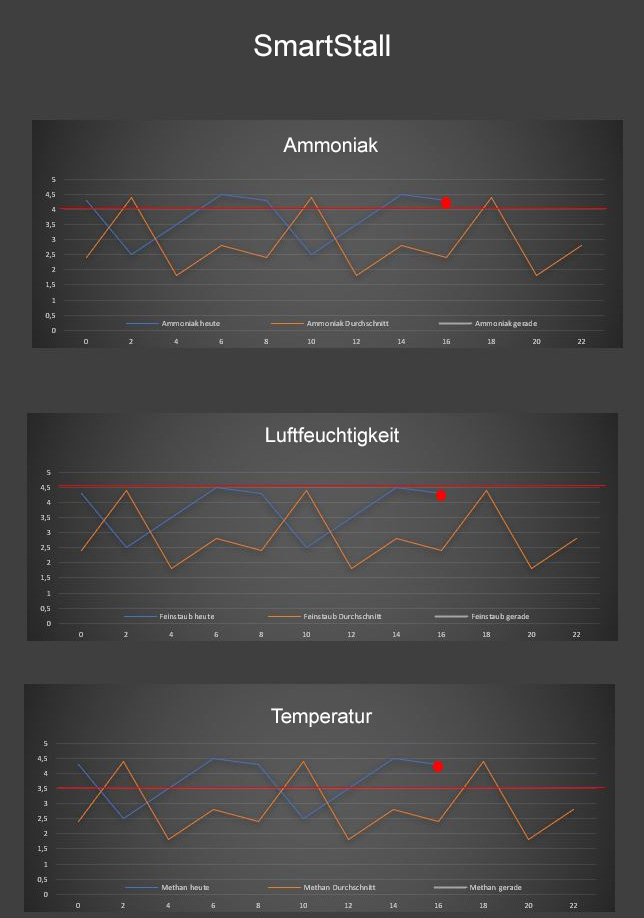
\includegraphics[width=80mm]{fig/firstUI.JPG}
	\caption{Erstentwurf eines möglichen Userinterfaces für die Webanwendung von SmartStall nach den ursprünglichen Überlegungen}
	\label{firstUI}
\end{figure}
Der Landwirt soll außerdem eine Push-Benachrichtigung auf dem Smartphone erhalten, wenn ein Schwellwert überschritten wird, und die Belüftung soll automatisch eingeschaltet werden. Sobald alle Werte unter den Schwellwerten liegen, soll die Belüftung wieder ausgeschaltet werden. \\
Es ist von großer Bedeutung, dass die Werte für Ammoniak, Luftfeuchtigkeit und Temperatur in einem Stall nicht zu hoch sind. Hohe Ammoniakkonzentrationen können die Atemwege der Tiere und Menschen reizen und zu ernsthaften gesundheitlichen Problemen führen \cite{ammoniak}. Eine zu hohe Luftfeuchtigkeit kann das Wachstum von Schimmel und anderen schädlichen Mikroorganismen fördern, was wiederum die Gesundheit der Tiere beeinträchtigt \cite{luftfeuchtigkeit}. Extreme Temperaturen, ob zu hoch oder zu niedrig, können den Komfort und das Wohlbefinden der Tiere negativ beeinflussen, was zu Stress und einer verminderten Produktivität führen kann \cite{temperatur}. Daher ist die Überwachung und Regelung dieser Parameter essenziell für die Gesundheit und das Wohlbefinden der Tiere sowie für eine effiziente landwirtschaftliche Produktion. 

\subsection{Gespräch mit Landwirten}
Da SmartStall ein IT-Produkt für Landwirte mit Tierhaltungsbetriebe werden soll, wurde nach den ersten Überlegungen und der ersten Skizze ein Gespräch mit zwei verschiedenen Landwirten geführt. Der erste landwirtschaftliche Betrieb ist der Bauernhof Stenglein in Rothwind, der etwa 80 Kühe in einem Stall hält. Der zweite landwirtschaftliche Betrieb ist der Bauernhof der Familie Stark aus Eichberg, die in der Ferkelerzeugung tätig sind. Beide reagierten positiv auf die Idee von SmartStall und fanden die Grundidee gut, brachten jedoch einige Verbesserungsvorschläge und wichtige Anmerkungen ein: 
\begin{itemize}
\item Die Landwirte waren der Meinung, dass es wenig Sinn macht, die durchschnittlichen Werte der einzelnen Luftqualitätsdaten anzuzeigen, da diese wenig aussagekräftig sind. Als Beispiel nannten sie die Temperatur: Im Sommer ist diese sehr hoch, im Winter eher niedrig. Ein Mittelwert daraus liefert keine nützlichen Informationen im Vergleich zum aktuellen Wert. Der Mittelwert wäre nur dann sinnvoll, wenn der Stall das ganze Jahr über konstante Bedingungen hätte, wie gleiche Außentemperatur und gleiche Dauer von geöffneten bzw. geschlossenen Türen und Fenstern, was in der Praxis jedoch nicht vorkommt. Da die Stalltüren ab spätem Frühling meist bis Herbst fast durchgängig geöffnet sind, herrschen unterschiedliche Bedingungen im Stall. Aus diesem Grund kann der durchschnittliche Wert der einzelnen Daten aus den Diagrammen entfernt werden, was zusätzlich die Lesbarkeit der Diagramme verbessert.
\item Den Landwirten war es außerdem wichtig, dass sie die Steuerung der Belüftung und die Push-Benachrichtigungen kontrollieren können. Da es sich um ein erstmaliges Projekt handelt, das noch nicht im Einsatz war, möchten sie sich nicht vollständig auf das System verlassen und die Möglichkeit haben, wie gewohnt vorzugehen. 
\item Ein weiterer Verbesserungsvorschlag war das Hinzufügen des aktuellen Werts zu jedem Diagramm, dam auf einen Blick der aktuelle Zustand im Stall erkannt werden kann.
\item Da der Bauernhof der Familie Stenglein recht groß ist und auch Angestellte im Stall arbeiten, die wenig Berührungspunkte mit Technik haben und nicht gut Deutsch sprechen, war es ihnen wichtig, dass die Anwendung simpel gehalten wird, damit sie jeder bedienen und verstehen kann.
\end{itemize}
\subsection{Überarbeitete Anforderungen}
Nach Abstimmungen mit den genannten Landwirten sehen die Anforderungen an das Projekt SmartStall wie folgt aus: \\
Die Luftqualitätsdaten des Stalls werden über einen Raspberry Pi in eine Datenbank geschrieben. Diese Daten werden in einer passwortgeschützten Webanwendung visualisiert, die drei verschiedene Diagramme enthält: eines für Ammoniak, eines für Luftfeuchtigkeit und eines für Temperatur. Die Diagramme zeigen die aktuellen Werte des Tages bzw. der letzten sieben Tage an. Die durchschnittlichen Werte für Tag und Woche wurden entfernt, um die Lesbarkeit zu verbessern.
Neben den Diagrammen wird der aktuelle Wert angezeigt, der in roter Schrift dargestellt ist, wenn der Wert die schädliche Grenze überschreitet, und in grüner Schrift, wenn er im unkritischen Bereich liegt. Es gibt außerdem zwei Schalter, mit denen die Automatisierung der Belüftung und das Benachrichtigen per Push-Nachricht bei Überschreitung des Grenzwerts aktiviert werden können.
Die Push-Benachrichtigungen werden an eine Telegram-Gruppe gesendet, in die alle Mitarbeiter eines Bauernhofs aufgenommen werden können, sodass alle relevanten Personen informiert werden. Eine Benachrichtigung per Telegram wird auch dann gesendet, wenn die automatische, schwellwertgesteuerte Belüftung in der Benutzeroberfläche der Webanwendung deaktiviert wird. Hierbei schaltet die Webanwendung die Smart-Steckdose und somit die Belüftung aus und informiert alle Mitglieder der Telegramm Gruppe darüber. Dies verhindert, dass die Belüftung unnötig lange läuft, falls sie zum Zeitpunkt der Deaktivierung noch aktiv ist, und trägt dazu bei, den Energieverbrauch des Stalls zu reduzieren. In Abschnitt \ref{ui} wird genauer auf die finale Benutzeroberfläche eingeangen.

\section{Aufbau und Zusammenspiel der Komponenten}
In diesem Kapitel werden die einzelnen Komponenten beleuchtet und es wird auf deren Zusammenspiel im Kontext dieses Projekts eingegangen. In Anhang \ref{sec:AufbauAnhang} ist ebenfalls eine Skizze des Aufbaus zu finden. \\
Angefangen bei der Datenerfassung stehen die Sensoren, die verschiedene Parameter zur Luftqualität messen. Diese Sensoren sind über das I2C-Protokoll mit einem Raspberry Pi verbunden, der als zentrale Steuerungseinheit fungiert. Auf die genauen Modelle der Hardwarekomponenten wird anschließend in Kapitel \ref{chapter:hw_komponenten} eingegangen. \\
Der Raspberry Pi sammelt kontinuierlich die Daten von den Sensoren und verarbeitet diese über ein Python-Skript weiter. Die gesammelten Daten werden über einen WLAN-Router, welcher die Verbindung zum Internet herstellt per HTTP-Protokoll an eine, über den Anbieter Oracle Cloud gehostete, Webanwendung weitergeleitet. Auf dem Webserver wird außerdem eine MYSQL-Datenbank gehostet und an die Webanwendung angebunden. Mit Hilfe dieser Anbindung können die Daten von der Webanwendung in die Datenbank weitergeleitet und dort gespeichert werden. \\
Die Webanwendung in der Oracle Cloud ermöglicht es Benutzern, über eine Weboberfläche auf die Daten zuzugreifen. Dies kann über den Browser eines beliebigen Endgeräts erfolgen. Neben der reinen Datenanzeige bietet die Webanwendung auch die Möglichkeit, Benachrichtigungen und Warnungen über den Telegram Messenger zu versenden. Diese Benachrichtigungen informieren die Benutzer in Echtzeit über kritische Zustände, wie beispielsweise hohe Ammoniakkonzentrationen. \\
Ein weiterer wichtiger Aspekt des Systems ist die Steuerung der Belüftungsanlage im SmartStall. Basierend auf den erfassten Sensordaten kann die Webanwendung die Belüftungsanlage über eine Smart-Steckdose automatisch ansteuern und die Belüftung somit ein- oder ausschalten sobald ein beliebiger Schwellwert eines Parameters, wie beispielsweise der Ammoniakgehalt, überschritten wird. 


\section{Hardware Komponenten}
\label{chapter:hw_komponenten}
\subsection{Raspberry Pi 3B}
Der Raspberry Pi (Modell 3B) ist ein beliebter Einplatinencomputer, der von der Raspberry Pi Foundation entwickelt wurde. Er bietet ausreichend Rechenleistung, Speicher und Konnektivität, um komplexe Aufgaben auszuführen und eine Vielzahl von Erweiterungen und Anwendungen zu unterstützen und ist somit eine kostengünstige und vielseitige Plattform für Projekte im Bereich der Einbettung von Computern und des IoT--Konzepts. Die umfangreiche Community und Dokumentation rund um den Raspberry Pi machen es einfach, Projekte zu starten und Unterstützung zu erhalten. Es gibt eine Vielzahl von Erweiterungsmodulen und Zubehörteilen, die den Raspberry Pi erweitern und an individuelle Anforderungen anpassen können \cite{raspy}. Um den Raspberry Pi 3B zu nutzen, ist eine grundlegende Einrichtung erforderlich, auf welche in Kapitel \ref{pi} genauer eingegangen wird.

\subsection{Bosch Sensortec BME680 Sensor}
Der Bosch Sensortec BME680 ist ein Umweltsensor, der verschiedene Messungen in einer kompakten Einheit vereint. Der BME680 Sensor ermöglicht die Messung von vier Umweltparametern:
\begin{itemize}
	\item Temperatur: Der Sensor misst die Umgebungstemperatur mit hoher Präzision.
	\item Luftfeuchtigkeit: Er erfasst die relative Luftfeuchtigkeit und liefert genaue Feuchtigkeitswerte.
	\item Luftdruck: Der Sensor kann den atmosphärischen Druck messen und damit Wettervorhersagen ermöglichen.
	\item Luftqualität: Der BME680 Sensor ist in der Lage, flüchtige organische Verbindungen (VOCs) und verschiedene Gase wie Kohlenmonoxid (CO) und Stickstoffdioxid (NO2) zu erkennen.
\end{itemize}
Der BME680 Sensor findet Anwendung in einer Vielzahl von Bereichen, wie beispielsweise der Erfassung von Wetterdaten in Außenbereichen und der Überwachung von Luftqualität in Innenräumen \cite{bme} \cite{bmeDataSheet}. 
\subsection{MQ137 NH3-Gassensormodul}
Das MQ137 Gassensor-Modul ist ein Sensor, der speziell entwickelt wurde, um Ammoniakgas (NH3) in der Umgebungsluft zu messen. Er basiert auf der Metalloxid-Gassensortechnologie und erfasst die Konzentration von Ammoniak in Parts per Million (ppm). Der Sensor reagiert auf das Vorhandensein von Ammoniak, indem er Änderungen in der elektrischen Leitfähigkeit erkennt. Das MQ137 Gassensor-Modul ermöglicht eine präzise Erfassung von Ammoniakgas und findet Anwendung in verschiedenen Bereichen wie Industrie, Landwirtschaft und Umweltüberwachung \cite{mqDataSheet}. Dieser Sensor wurde gewählt, da er eine kosteneffiziente Alternative zu komplexeren hochpreisigen Sensoren darstellt, welche neben Ammoniak weitere Parameter messen, die für den Kontext der Luftqualitätsüberwachung in einem Stall allerdings nicht benötigt, oder bereits durch den BME680 Sensor abgedeckt werden.

\subsection{Verbinden der Komponenten}
Um die vorgestellten Sensoren nutzen zu können, müssen diese an die korrekten Pins des Raspberry Pis angeschlossen werden. Die zur Verfügung stehenden Pins des Raspberry Pis sind in Abbildung \ref{pi_pins} dargestellt.

\begin{figure}[H]
	\centering
	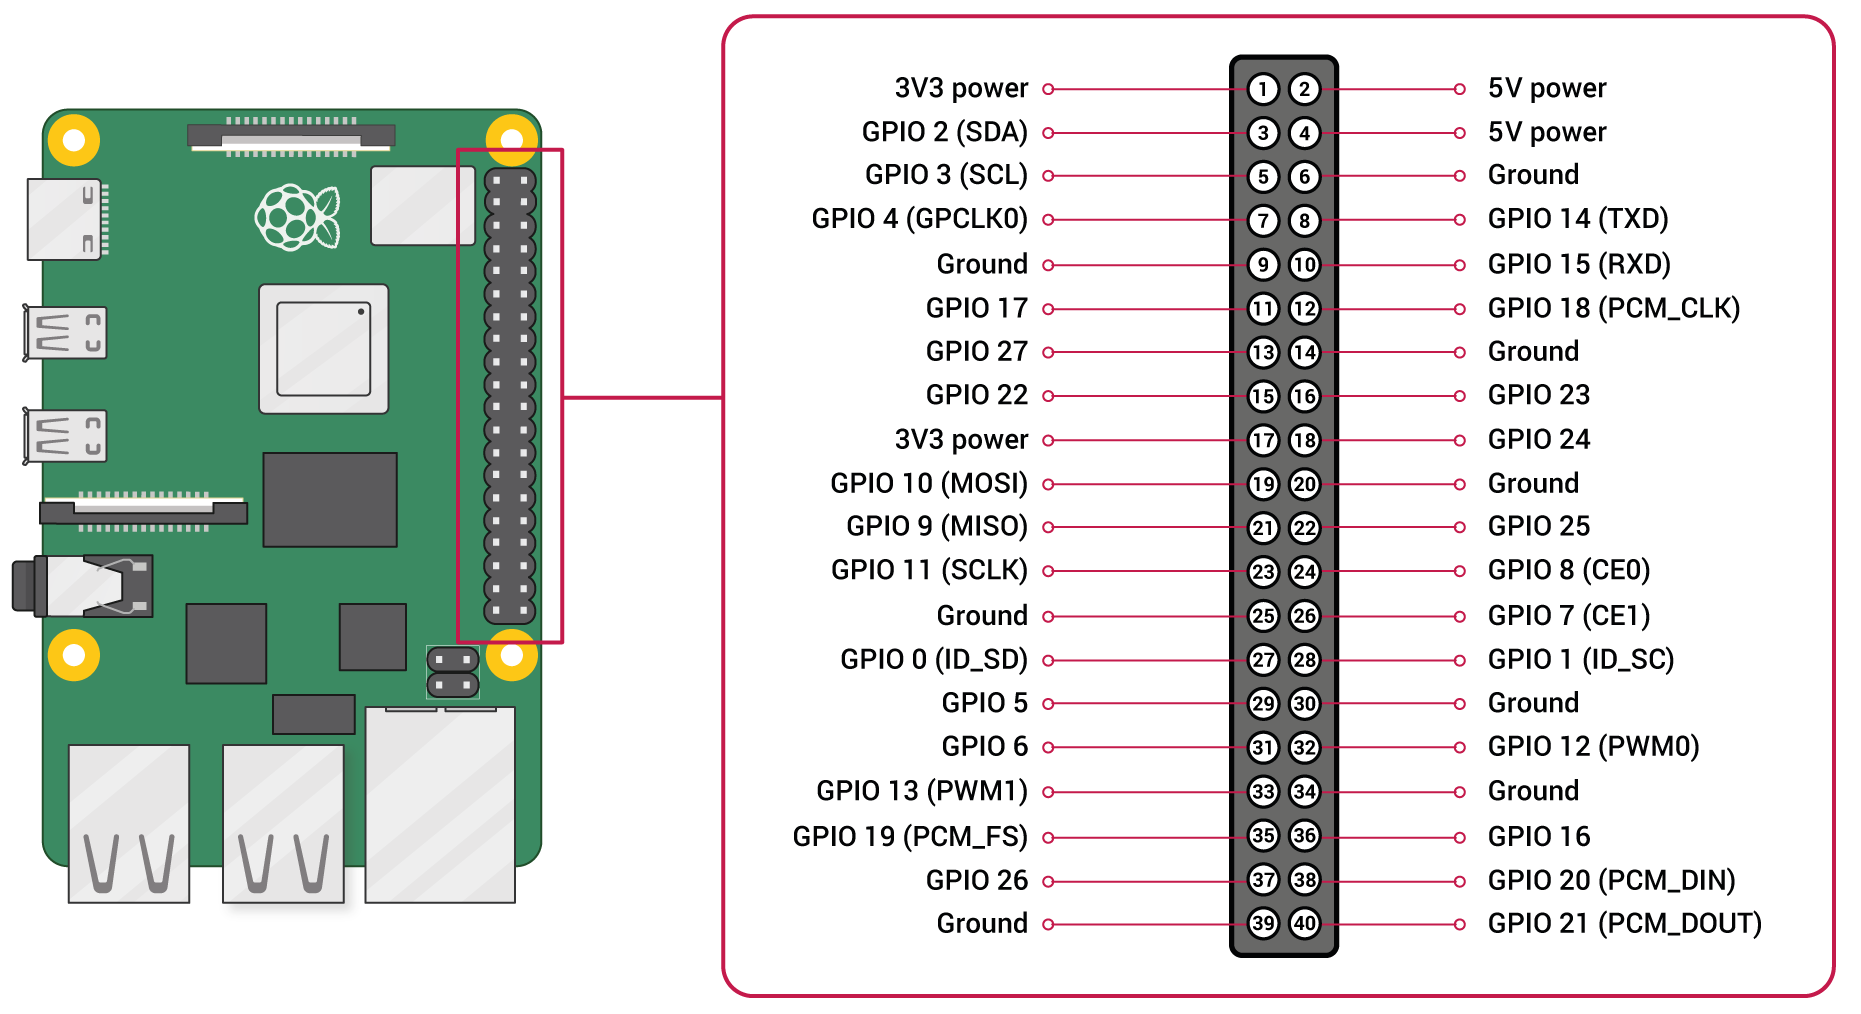
\includegraphics[width=90mm]{fig/pi_pins.png}
	\caption{Raspberry Pi 3B Pin Belegung \cite{bmeAbbildungen}}
	\label{pi_pins}
\end{figure}

\subsubsection{Anschließen des BME680 Sensors} 


Der BME680 besitzt sechs Pins, welche Abbildung \ref{bme_pins} zu entnehmen sind. Relevant sind hierbei die oberen 4 Pins, welche wie in Abbildung \ref{verkabelung_bme} aufgezeigt, an den Raspberry Pi angeschlossen werden müssen. \cite{bme_anschluss}
\begin{figure}[H]
	\centering
	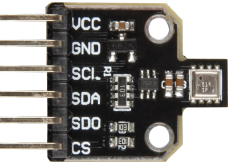
\includegraphics[width=50mm]{fig/bme_pins.png}
	\caption{BME680 Pins}
	\label{bme_pins}
\end{figure}
\begin{figure}[H]
	\centerline{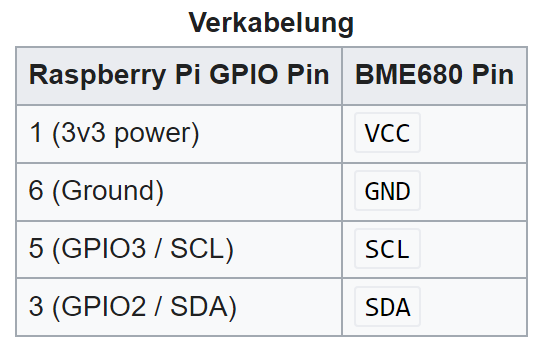
\includegraphics[width=50mm]{fig/verkabelung_bme.png}}
	\caption{Pin Verbindungen von Raspberry Pi und BME680 \cite{bmeAbbildungen}}
	\label{verkabelung_bme}
\end{figure}
Über die Pins VCC und GND wird die Stromversorgung des BME680 über den Raspberry Pi sichergestellt. Für die Datenübertragung wird die sogenannte Inter-Integrated-Circuit Schnittstelle (I$^2$C) genutzt. I$^2$C ist ein synchrones, serielles Kommunikationsprotokoll, das über zwei Leitungen eine bidirektionale Kommunikation zwischen einem oder mehreren Master- und Slave-Geräten ermöglicht. Der SDA Pin dient hierbei als Datenleitung und der SCL Pin ist für die Übertragung des Takts für die Datenübertragung zuständig. Die Datenübertragung funktioniert nach dem Master-Slave-Prinzip, es gibt ein Master-Gerät, welches die Kommunikation initiiert und den Takt vorgibt, in diesem Fall der Raspberry Pi und ein oder mehrere Slave-Geräte, welche auf die Befehle des Masters reagieren, in diesem Fall der BME680 Sensor \cite{i2cDoc}. \\

\subsubsection{Anschließen des MQ137 Sensors} 
Der MQ137 Sensor besitzt, wie in Abbildung \ref{mq137_pins} zu sehen, 4 Pins, welche ebenfalls mit den jeweiligen Pins des Raspberry Pis verbunden werden müssen:
\begin{itemize}
	\item VCC: Stromversorgung (5V)
	\item GND: Ground
	\item DO: digitaler Signalausgang
	\item AO: analoger Signalausgang
\end{itemize}
\begin{figure}[H]
	\centerline{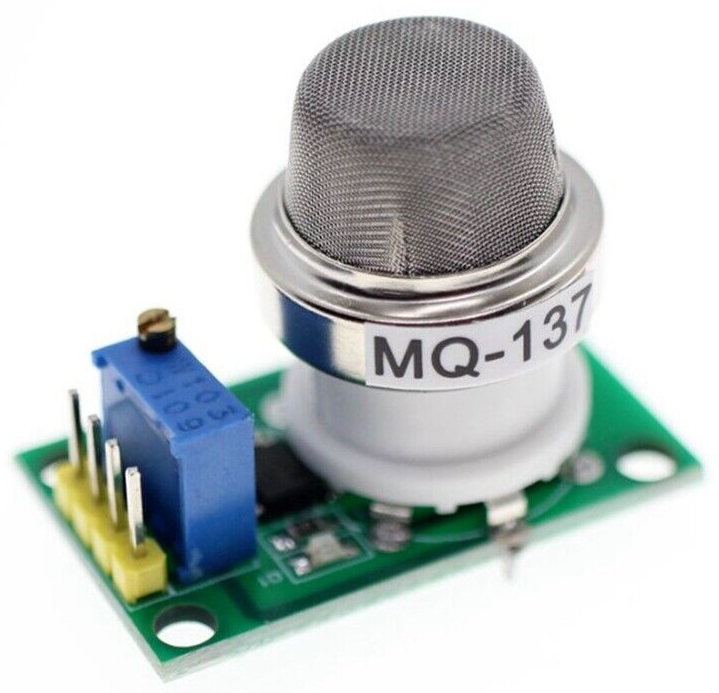
\includegraphics[height=25mm]{fig/mq137_pins.png}}
	\caption{MQ137 Gassensormodul}
	\label{mq137_pins}
\end{figure}
Um den MQ137 Sensor mit Strom zu versorgen und zunächst über den digitalen Output Pin an den Raspberry Pi ein High bzw. Low Signal senden zu können, je nachdem ob ein bestimmter Schwellwert von Ammoniak gemessen wird oder nicht, müssen folgende Pins zwischen Raspberry Pi und MQ137 Sensor verbunden werden:
\begin{table}[h!]
	\centering
	\begin{tabular}{|p{4cm}|p{4cm}|}
		\hline
		\textbf{Raspberry Pi GPIO Pin} & \textbf{MQ-137 Pin} \\
		\hline
		3 (5V power) & VCC \\
		\cline{1-2}
		6 (Ground) & GND \\
		\cline{1-2}
		38 (GPIO20 / PCM\_DIN) & DO \\
		\hline
	\end{tabular}
	%\caption*{Pin-Verbindungen zwischen Raspberry Pi und MQ-137}
\end{table}

\newpage
\subsubsection{Gesamtaufbau}
Die Sensoren wurden mittels Jumper-Kabeln und einem Breadboard mit dem Raspberry Pi verbunden. Der Aufbau und die beschriebene Verkabelung der Sensoren mit dem Raspberry Pi ist Abbildung \ref{aufbau} zu sehen.
\begin{figure}[htbp]
	\centerline{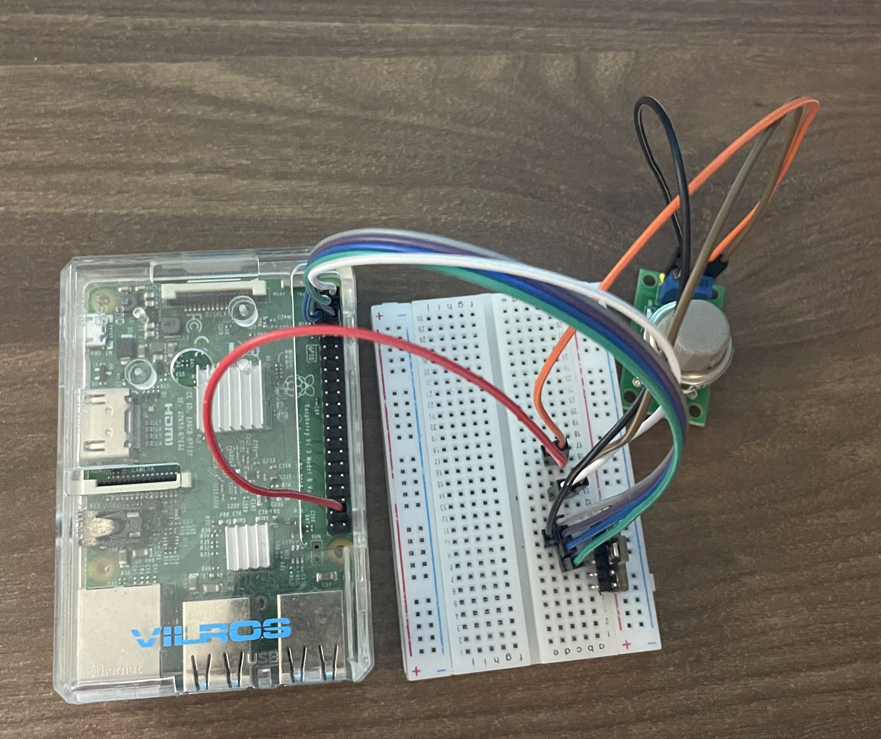
\includegraphics[width=80mm]{fig/aufbau.png}}
	\caption{Verkabelung der Sensoren mit dem Raspberry Pi}
	\label{aufbau}
\end{figure}

\section{Einrichtung Raspberry Pi}
\label{pi}
\subsection{Konfiguration}
Die erstmalige Einrichtung eines Raspberry Pi 3B umfasst mehrere Schritte, welche in diesem Kapitel aufgelistet werden. Zunächst eine Auflistung der benötigten und in diesem Projekt verwendeten Komponenten:
\begin{itemize}
	\item Raspberry Pi 3B
	\item MicroSD-Karte (mindestens 8 GB)
	\item Netzteil (5V)
	\item USB-Tastatur und -Maus
	\item HDMI-Kabel
	\item Bildschirm oder Fernseher mit HDMI-Eingang
\end{itemize}

Wenn das Anschließen von Ein- und Ausgabegeräten an den Raspberry Pi nicht gewünscht oder möglich ist, kann dieser nach der ersten Einrichtung alternativ auch über einen anderen Computer angesteuert werden, entweder per Remotedesktopverbindung oder per Kommandozeile mit Hilfe des Secure Shell (SSH) Netzwerkprotokolls \cite{raspy}. Zur erstmaligen Einrichtung muss zunächst das gewünschte Betriebssystem für den Raspberry Pi heruntergeladen werden, in diesem Fall Raspbian. Hierfür wurde das Program Raspberry Pi Imager von der offiziellen Raspberry Pi Website verwendet, welches die ausgewählte Version des Betriebssystems herunterlädt und diese direkt auf der MicroSD-Karte installiert. Anschließend kann die MicroSD-Karte in den Raspberry Pi eingesetzt und dieser gestartet werden. Für die Einrichtung muss nun lediglich den Anweisungen auf dem Bildschirm gefolgt werden, anschließend kann der Raspberry Pi über die grafische Benutzeroberfläche verwendet oder über Konsole angesteuert werden.  


\subsection{Software und Bibliotheken}
Nach der Einrichtung des Raspberry Pi musste zunächst das I2C (Inter-Integrated Circuit) Interface über die raspi-config aktiviert werden. I2C  ist ein serieller Kommunikationsbus zur Verbindung von elektronischen Bauteilen über nur zwei Datenleitungen: SDA (Serial Data Line) und SCL (Serial Clock Line). Es ermöglicht die einfache Kommunikation zwischen verschiedenen Geräten wie Mikrocontrollern, Sensoren und Aktoren. Dieser wird vom BME680 Sensor zur Übertragung der Messwerte genutzt. Da für das Abfragen der Sensordaten in diesem Projekt Python verwendet wird, welches bereits standardmäßig mit dem Raspian Betriebssystem mitinstalliert wird, müssen zusätzlich noch einige Bibliotheken installiert werden: 
\begin{itemize}
	\item python3-smbus: \\
	Ermöglicht die Kommunikation über in I2C-Bus in Python. Es werden Funktionen bereitgestellt I2C-Geräte anzusprechen und Daten zu senden und zu empfangen.
	\item i2c-tools: \\
	 Wird für die Verwaltung und Diagnose des I2C-Busses verwendet. Dies bietet zusätzliche Funktionalitäten wie das Anzeigen angeschlossener Geräte.
	\item adafruit-circuitpython-bme680: \\
	Dies ist eine Bibliothek zur Kommunikation mit dem BME680 Sensor, welche die Interaktion mit dem Sensor ermöglicht, um Sensordaten auszulesen und die Messgenauigkeit zu beeinflussen.
	\item rpi.gpio: \\
	Hierbei handelt es sich um eine Bibliothek, welche für die Konfiguration und Überwachung der GPIO-Pins des Raspberry Pis entwickelt wurde. Sie wird in diesem Kontext verwendet um einen Pin als digitalen Eingang zu konfigurieren, um das digitale Out Signal des MQ137 Sensors auszulesen.
\end{itemize}

\subsection{Datenübertragung}
\label{chapter:datenuebertragung}
Die Datenübertragung vom Raspberry Pi an die Webanwendung findet über ein Python-Skript statt. Python bietet sich hierbei als Programmiersprache aufgrund der knappen und prägnanten Syntax an und ist außerdem auf dem Betriebssystem des Raspberry Pi vorinstalliert, sodass kein zusätzlicher Aufwand nötig ist, um das Skript zum laufen zu bringen. Ein weiterer Vorteil von Python ist die Plattformunabhängigkeit, wodurch die Datenübertragung ebenfalls auf anderen Betriebssystemen wie Windows, Linux und MacOS problemlos ohne Änderungen ausgeführt werden könnte. \\
Das Skript dient dazu, die von den Sensoren gemessenen Daten zu erfassen, entsprechend zu formatieren und an die Webanwendung zu senden. Es beginnt mit der Initialisierung und Erkennung der Sensoren. Das Skript versucht, den BME680 Sensor unter der primären I2C-Adresse zu initialisieren. Wird der Sensor erkannt, werden verschiedene Parameter wie Oversampling und Filtergröße konfiguriert, um genaue Messungen zu gewährleisten. Unter Oversampling versteht man die Anzahl der Messungen zu einem Messzeitpunkt, um anschließend den Durchschnittswert zu berechnen und so die Genauigkeit der Messung zu erhöhen. Filtergröße bezieht sich auf den digitalen Filter, der verwendet wird, um Rauschen und kleine Schwankungen in den Sensordaten zu glätten. Der Filter reduziert die Auswirkungen von plötzlichen Änderungen oder Rauschen, indem er eine gleitende Durchschnittsberechnung anwendet. \\
Zusätzlich wird der MQ137-Sensor konfiguriert. Der digitale Ausgangspin dieses Sensors wird angesteuert, und es wird überprüft, ob der Sensor erreichbar ist. \\
Im nächsten Schritt erfasst das Skript die Sensordaten und sendet sie per HTTP-Anfrage an die Webanwendung. Hierbei werden die aktuellen Sensorwerte ausgelesen und in ein JSON-Objekt verpackt. Dieses Objekt wird dann über eine vordefinierte Route mit der entsprechenden URL an die Webanwendung gesendet. Das Skript überprüft anschließend, ob die Übertragung erfolgreich war und gibt entsprechend eine Erfolgsmeldung oder eine Fehlermeldung zurück, falls der Raspberry Pi nicht mit dem Internet verbunden, oder die Webanwendung nicht erreichbar ist. Diese Meldungen werden zusammen mit den Sensordaten in einer Log-Datei gespeichert. Ein beispielhafter Log-Eintrag für eine erfolgreiche Datenübertragung ist in Abbildung \ref{send_data_success} zu sehen. Zum Abschluss werden die verwendeten GPIO-Pins bereinigt, um sicherzustellen, dass keine Ressourcen unnötig belegt bleiben.
\begin{figure}[H]
	\centering
	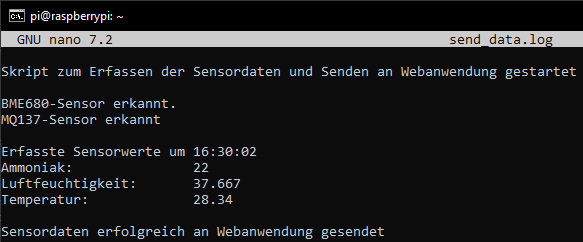
\includegraphics[width=85mm]{fig/daten_erfolgreich_gesendet.png}
	\caption{Logeintrag für erfolgreich gesendete Sensordaten}
	\label{send_data_success}
\end{figure}
Um Ressourcen zu schonen, enthält das Skript keine Schleife, die die Daten in regelmäßigen Abständen ausliest und sendet. Stattdessen wird das Skript nach der Ausführung, also der einmaligen Datenübertragung, zunächst beendet. Für die regelmäßige Ausführung des Skripts wird Crontab genutzt. \\ 
Crontab ist ein Dienst auf Unix-basierten Betriebssystemen, der es ermöglicht, Aufgaben zu einem bestimmten Zeitplan auszuführen. Es handelt sich um eine Zeitplanungsdatei, die als Crontab-Datei bezeichnet wird und in der definiert wird, wann und wie oft bestimmte Befehle oder Skripte automatisch ausgeführt werden sollen \cite{crontab}. Die Verwendung von Crontab zur regelmäßigen Ausführung eines Python-Skripts in festgelegten Intervallen bietet mehrere Vorteile. Diese umfassen eine effizientere Nutzung der Systemressourcen, eine vereinfachte Verwaltung und Fehlerbehebung sowie eine erleichterte Systemwartung. Ein dauerhaft laufendes Skript verbraucht kontinuierlich Speicher, selbst wenn es inaktiv ist. \\
Crontab startet das Skript nur bei Bedarf, wodurch der Speicherverbrauch erheblich reduziert wird und die Systemressourcen effizienter genutzt werden. Darüber hinaus erleichtert Crontab die Verwaltung und das Debugging. Jedes Mal, wenn das Skript neu startet, beginnt es in einem sauberen Zustand, was die Fehlersuche vereinfacht und die Stabilität erhöht. Fehler oder inkonsistente Zustände, die sich in einem dauerhaft laufenden Skript ansammeln könnten, werden durch den Neustart behoben. Ein weiterer Vorteil ist die automatische Handhabung von Systemwartungen. Während dauerhaft laufende Skripte nach einem Neustart manuell neu gestartet werden müssen, starten Crontab-Jobs automatisch, was die Wiederherstellung des Betriebs nach Wartung, Updates oder unerwarteten Neustarts erleichtert.

\section{Webanwendung}
\subsection{Architektur}
Die Webanwendung wurde mit dem ASP.NET Core Framework für C-Sharp, unter Verwendung der .NET-Plattform, entwickelt. ASP.NET Core ist ein modernes, plattformübergreifendes Framework für die Entwicklung von Webanwendungen. Es bietet eine modularisierte Architektur, die Entwicklern ermöglicht, nur benötigte Komponenten zu verwenden, was die Performance verbessert und die Anpassungsfähigkeit erhöht. Durch seine Plattformunabhängigkeit läuft ASP.NET Core auf Windows, macOS und Linux, was Flexibilität bei der Bereitstellung ermöglicht. Das Framework ist stark auf Performance optimiert und unterstützt moderne Webentwicklungsmuster \cite{dotNET} \cite{csharp}. \\
Ein Beispiel hierfür das Model-View-Controller, kurz MVC, welches für die Webanwendung verwendet wurde. Hierbei handelt es sich um ein moderneres Designmuster, das die Trennung von Datenmodell, Präsentationsschicht und Steuerungslogik fördert, was die Struktur und Übersichtlichkeit der Webanwendung verbessert.
\subsection{Hosting}
Die Webanwendung wird auf einem Oracle Cloud Webserver gehostet, der mit dem Linux-Betriebssystem läuft. Diese Entscheidung bietet mehrere Vorteile für das Projekt. Einerseits gewährleistet der Oracle Cloud Webserver eine hohe Zuverlässigkeit und Verfügbarkeit der Anwendung durch seine robuste Infrastruktur und Service Level Agreements. Außerdem besteht die Möglichkeit, Ressourcen nach Bedarf zu skalieren, dass die Anwendung problemlos mit steigenden Benutzeranforderungen wachsen kann. Diese Flexibilität unterstützt auch eine kosteneffiziente Nutzung, da Ressourcen nur dann erhöht werden, wenn sie auch tatsächlich benötigt werden. Für die Durchführung des Projekts wurde die sogenannte \textit{Oracle Cloud Free Tier} genutzt. \\
Hierbei handelt es sich um einen kostenlosen Tarif mit entsprechend eingeschränkter Rechenleistung. Da sich die zur Verfügung stehenden Ressourcen allerdings beliebig skalieren lassen, ist es jederzeit ohne Mehraufwand möglich zusätzliche Rechenleistung anzumieten, welche gegebenenfalls in der Zukunft bei Weiterentwicklung der Anwendung für zusätzliche Funktionen benötigt wird. Das Hosting auf einem Oracle Cloud Webserver bietet somit eine solide Grundlage für eine sichere, skalierbare und kosteneffiziente Bereitstellung der Webanwendung. \\
\subsection{Deployment}
Das Deployment einer ASP.NET Core Webanwendung auf einem Linux Webserver umfasst mehrere Schritte, um sicherzustellen, dass die Anwendung ordnungsgemäß bereitgestellt und ausgeführt wird. Dieses Kapitel erläutert den den Prozess vom Entwicklungs- bis zum Produktionsumfeld
Notwendige Schritte für das Deployment sind:
\begin{itemize}
	\item Vorbereitung der Entwicklungsumgebung: \\
	Zunächst wird die ASP.NET Core Webanwendung in der Entwicklungsumgebung entwickelt und getestet. Dies beinhaltet die Implementierung von Funktionen, das Testen der Anwendung und das Sicherstellen, dass sie fehlerfrei läuft.
	\item Kompilieren der Anwendung: \\
	Die ASP.NET Core Webanwendung muss in der Release Konfiguration vollständig kompiliert werden. Hierbei wird die Build-Funktionen von Visual Studio, der für das Projekt verwendeten Entwicklungsumgebung, genutzt.
	\item Erstellung eines Deployment-Pakets: \\
	Die Anwendung wird als Deployment-Paket veröffentlicht, das alle erforderlichen Dateien und Abhängigkeiten für die Ausführung auf einem Linux Webserver enthält. Das Paket wird im Projektordner mit einem .NET-SDK-Befehl erstellt. Dieser sieht folgendermaßen aus:\\
	\textit{dotnet publish -c Release -r linux-x64 --self-contained} \\
	Der Parameter \textit{--self-contained} wird verwendet um sicherzustellen, dass alle benötigten .NET Core Laufzeitdateien enthalten sind, mit dem Parameter \textit{-r linux-x64} wird die Zielplatform, in diesem Fall Linux 64-Bit spezifiziert. Durch die Ausführung des Befehls wird also ein Verzeichnis mit der kompilierten Anwendung und allen notwendigen Dateien für die Ausführung auf Linux erstellt.
	\item Einrichtung des Linux-Servers: \\
	Auf dem Ziel-Linux-Server werden die notwendigen Abhängigkeiten installiert, einschließlich des .NET Core Laufzeitumgebung und des gewählten Webservers, in diesem Fall Apache. Ein Apache Webserver ist eine Open-Source-Software, die für das Hosting von Webseiten und Webanwendungen am weitesten verbreitet ist. 
	\item Übertragung und Entpacken des Deployment-Pakets: \\
	Das erstellte Deployment-Paket wird auf den Linux-Server übertragen, entpackt und in das entsprechende Zielverzeichnis verschoben.
	\item Konfiguration des Webservers: \\
	Der Apache Webserver wird konfiguriert, um Anfragen an die ASP.NET Core Anwendung weiterzuleiten. Dies umfasst das Festlegen von Hostnamen, Portnummern und anderen relevanten Einstellungen in der Webserver-Konfigurationsdatei. Die Webanwendung kann somit über die IP-Adresse \textit{http://141.147.6.122/} über Port \textit{8081} erreich werden.
	\item Starten der Anwendung: \\
	Das Deployment Paket beinhaltet eine ausführbare \textit{.dll} Datei, welche von einer zusätzlich konfigurierten Linux Service-Datei automatisch beim Start des Webservers ausgeführt und somit die Webanwendung gestartet wird.
\end{itemize}
\subsection{Software Design}
Für die Webanwendung wurde die MVC Architektur angewendet. Dies ist eines der etablierten Architekturmuster und teil des verwendeten ASP.NET C\# Frameworks. Architekturmuster bzw. Patterns sind in der modernen Softwareentwicklung und -architektur von großer Bedeutung, da sie eine klar definierte Terminologie und eine saubere Dokumentation bieten.  \\
Das MVC-Muster ist besonders geeignet für interaktive Anwendungen, die eine flexible Schnittstelle zwischen Mensch und Maschine erfordern. MVC unterteilt die Programmlogik einer Benutzeroberfläche in drei Hauptkomponenten: Model, View und Controller. Das Model verwaltet die Daten und Geschäftsregeln der Anwendung. Die View stellt diese Daten dar, und der Controller ermöglicht die Interaktion mit dem Benutzer. \cite{mvc} \\
In diesem Projekt werden Models zur Datenhaltung zwischen dem Empfangen der Daten und dem Abspeichern in der Datenbank. Hierfür wurde beispielsweise ein Model \text{Datenpaket} erstellt, welches die einzelnen Sensordaten der drei betrachteten Parameter Temperatur, Luftfeuchtigkeit und Ammoniak in Variablen zwischenspeichert. Die View besteht aus der Login-Seite und der Hauptseite. Benutzer melden sich mit Passwort und Benutzernamen an, bevor sie zur Hauptseite gelangen, wo die Diagramme visualisiert werden. Im Controller sind zwei Funktionen besonders wichtig: \\
Der \textit{DbWriteService}, welcher das empfangene Datenpaket in die Datenbank schreibt und der \textit{DbReadService}, welcher die Sensordaten jeweils für eine Woche bzw. für einen Tag aus der Datenbank ausliest und diese an die Diagramme in der Benutzeroberfläche weitergibt. Die Kommunikation zwischen View und Controller erfolgt über AJAX-Aufrufe, wodurch die Sensordaten, wie in Kapitel \ref{sec:sensordaten-auslesen} beschrieben, abgerufen werden.
\newpage
\subsection{MYSQL Datenbank}
\subsubsection{Anbindung}
Die Anbindung einer MySQL-Datenbank in der ASP.NET Core Webanwendung erfolgt über das Entity Framework Core von Microsoft, welches zunächst in der Entwicklungsumgebung installiert werden muss. Anschließend werden Verbindungsdaten wie Hostname, Benutzername, Passwort und Datenbankname der gehosteten Datenbank benötigt. Die Verbindung wird als sogenannter \textit{ConnectionString} in einer separaten Konfigurationsdatei der Webanwendung definiert. Dieser sieht wie folgt aus: \\
\begin{verbatim}
"DefaultConnection": "Server=localhost;
Database=MeinDatenbankName;
User=root;Password=MeinPasswort;"
\end{verbatim}
Die Webanwendung kann sich mit Hilfe des entsprechenden Frameworks und den Zugangsdaten mit der Datenbank verbinden und Anweisungen, sogenannte SQL-Querys in Form von Strings senden, welche der MYSQL-Syntax entsprechen müssen. Die Query-Strings können anschließend einem Objekt der Klasse \textit{MySqlCommand} zugewiesen und über dieses an die Datenbank übermittelt werden.
\subsubsection{Tabellenstruktur}
Der Aufbau der Datenbanktabelle \textit{sensordata} ist einfach gehalten. In diese Tabelle werden die Sensordaten über den entsprechenden Service eingefügt. Die Tabelle enthält unter anderem einen Zeitstempel, der als Primary Key fungiert. Ein Primary Key in einer Datenbank ist ein spezielles Feld oder eine Kombination von Feldern, das jeden Datensatz in einer Tabelle eindeutig identifiziert und keine NULL-Werte enthalten darf. Die Sensorwerte für Ammoniak, Luftfeuchtigkeit und Temperatur werden jeweils als Gleitkommazahlen in der Datenbank gespeichert. Die Spalten und Datentypen der Tabelle \textit{sensordata} ist im Folgenden zu sehen:
\begin{table}[h!]
    \centering
    \begin{tabular}{|c|c|c|}
        \hline
        \textbf{Spaltenname} & \textbf{Datentyp}  & \textbf{Bedingung} \\
        \hline
        timestamp & timestamp & PRIMARY KEY \\
        \hline
        ammoniak & float & \\
        \hline
        luftfeuchtigkeit & float &  \\
        \hline
        temperatur & float & \\
        \hline
    \end{tabular}
    \label{tab:sensordata}
\end{table}
\subsection{API-Schnittstelle zum Empfangen und Speichern der Daten}
Um die vom Raspberry Pi gesendeten Daten zu empfangen und diese in die MYSQL-Datenbank einzufügen, sind unterschiedliche Schritte notwendig. Zunächst muss ein Endpunkt erstellt werden, welcher eine Route definiert. Dieser enthält eine Unterseite der Webanwendung, welche von der HTTP-Post Anfrage angesteuert werden muss und einen Controller, welcher die ankommenden Daten empfängt und weiterverarbeitet. Die Sub-URL, auf welche der Controller hört, lautet \textit{http://141.147.6.122:8081/ReceiveData} \\
Der Controller ruft anschließend einen Service auf, welcher eine Funktion enthält, die dafür sorgt, dass die empfangenen Sensordaten in der Datenbank gespeichert werden. Der genaue Ablauf der Funktion sieht folgendermaßen aus:
\begin{itemize}
	\item Datenbankverbindung: \\
	Die Funktion beginnt mit der Herstellung einer Verbindung zur MySQL-Datenbank. Dafür wird der im vorherigen Kapitel erwähnte ConnectionString verwendet.
	\item Vorbereitung der SQL-Abfrage: \\
	Eine SQL-INSERT-Abfrage wird vorbereitet, um die empfangenen Daten in die entsprechende Tabelle der Datenbank einzufügen. Die Abfrage enthält Platzhalter für die einzelnen Werte des Datenpaket, um eine sichere Parameterübergabe zu gewährleisten und SQL-Injections zu verhindern.
	\item Parameterübergabe: \\
	Die Werte werden den Platzhaltern der SQL-Abfrage zugewiesen. Dies umfasst den Zeitstempel sowie die Sensorwerte für Temperatur, Luftfeuchtigkeit und Ammoniak.
	\item Ausführen der Abfrage: \\
	Die vorbereitete und mit Parametern versehene SQL-Abfrage wird ausgeführt, wodurch die Daten in die Tabelle eingefügt werden.
	\item Fehlerbehandlung: \\
	Während der gesamten Operation wird ein try-catch-Block verwendet, um mögliche Fehler abzufangen. Wenn ein Fehler auftritt, wird dieser im catch-Block behandelt und eine entsprechende Fehlermeldung wird ausgegeben.
\end{itemize}


\subsection{Auslesen und Anzeigen der Sensordaten}
\label{sec:sensordaten-auslesen}
Für die Anzeige der Sensordaten in der Webanwendung wurden bestimmte Anforderungen definiert. Zum einen sollten die Daten in einem Liniendiagramm dargestellt werden, und zum anderen sollte die Webanwendung sowohl auf PCs und Laptops als auch auf mobilen Geräten reibungslos funktionieren. Um dieses Problem zu lösen wurde das Bootstrap Framework gewählt.\\
Bootstrap besitzt eine breite Palette an vorgefertigten UI-Komponenten und bietet ein Grid-System, welches sich responsive gegenüber unterschiedlichen Bildschirmgrößen und Auflösungen auf verschiedenen Endgeräten verhält. Dies ermöglicht eine einfache Integration und schnelle Entwicklung von modernen und benutzerfreundlichen Webseiten, unabhängig vom verwendeten Gerät \cite{bootstrap}. \\
Um Bootstrap effektiv zu nutzen, wurden folgende JavaScript-Bibliotheken integriert: 
\newpage
\begin{itemize}
\item jQuery: \\
Diese leistungsstarke Bibliothek unterstützt die Manipulation des DOM und erleichtert AJAX-Interaktionen. In Verbindung mit Bootstrap ermöglicht sie die dynamische Aktualisierung von Inhalten und die Interaktion mit Benutzeroberflächenelementen wie Dropdown-Menüs oder Modalfenstern.
\begin{verbatim}
<script src="https://code.jquery.com/
jquery-3.6.0.min.js"></scrip
\end{verbatim}
\item Popper.js: \\
Diese Bibliothek wird verwendet, um Popups, Tooltips und Dropdown-Menüs präzise innerhalb einer Bootstrap-Anwendung zu positionieren. Dies verbessert die Benutzerfreundlichkeit und sorgt für eine optimale Platzierung basierend auf dem verfügbaren Bildschirmraum. In der Webanwendung wird Poppers.js verwendet, um an spezifischen Datenpunkten in den Diagrammen den Zeitstempel und Wert des Parameters anzeigen zu können.
\begin{verbatim}
<script src="https://cdn.jsdelivr.net/
npm/popper.js@1.16.1/dist/umd/popper.min.
js"></script>
\end{verbatim}
\item Bootstrap: \\
Das Bootstrap-Bundle enthält das Haupt-JavaScript von Bootstrap. Dieses Framework bietet Funktionen wie responsives Design, Grid-Systeme und Modalkomponenten, die für die Implementierung des Liniendiagramms und anderer UI-Elemente essentiell sind.
\begin{verbatim}
<script src="https://cdn.jsdelivr.net/
npm/bootstrap@4.6.2/dist/js/bootstrap.
bundle.min.js"></script>
\end{verbatim}
Zusammen stellen diese Skript-Links sicher, dass Bootstrap nahtlos in die Webanwendung integriert wird und eine optimale Benutzerinteraktion sowie eine responsive Darstellung auf verschiedenen Geräten gewährleistet ist. \\
\item Chart.js: \\
Für die Darstellung der Sensordaten in einem Liniendiagramm wurde Chart.js gewählt. Diese Bibliothek bietet eine einfache und flexible Möglichkeit, Daten visuell ansprechend darzustellen. Im Vergleich zu Grafana, das eher für umfangreichere und komplexe Datenvisualisierungen in großen Systemen verwendet wird \cite{grafana}, ist Chart.js leichter in kleinere Webanwendungen zu integrieren und bietet dennoch ausreichend Funktionalität für die Anforderungen der Sensordatenvisualisierung \cite{chart.js}. \\
Die folgenden Links integrieren Chart.js und das zugehörige Datum-Adapter-Bundle in die Webseite:
\begin{verbatim}
<script src="https://cdn.jsdelivr.net/npm/
chart.js"></script>
<script src="https://cdn.jsdelivr.net/npm
/chartjs-adapter-date-fns/dist/chartjs-
adapter-date-fns.bundle.min.js"></script>
\end{verbatim}
\end{itemize}
Die Kombination der gennanten Bibliotheken ermöglichen eine effektive und effiziente Darstellung der Sensordaten in der Webanwendung, optimiert für verschiedene Geräte und Benutzerumgebungen.
Nachdem die benötigten Bibliotheken eingebunden wurden, können die Diagramme in der Webanwendung aufgebaut werden. Der  HTML-Code in Anhang \ref{sec:htmlCodeDiagrammAnhang} definiert die Struktur eines Diagramms inklusive dem aktuellen Wert anhand der Temperatur. \\
Das eigentliche Diagramm wird durch das \textit{\textless canvas\textgreater{}}-Element mit der ID \textit{lineChartTemperatur} dargestellt. Mir dieser ID kann genau dieses Diagramm bearbeitet werden.
Um die Sensordaten für beispielsweise die Temperatur abzurufen, wird AJAX verwendet. AJAX ermöglicht es, Daten asynchron im Hintergrund zu laden, ohne die gesamte Webseite neu zu laden. Der JavaScript-Code in Anhang \ref{sec:ajaxAnhang} zeigt einen Beispielaufruf. \\
Hierbei ist \textit{GetTemperatur} die URL, unter der die Sensordaten abgerufen werden. Hinter dieser URL steckt eine Funktion, die im C\#-Code in dem \textit{HomeController} implementiert ist. Diese Funktion bzw. der Service \textit{DbReadService} ist dafür zuständig, alle Daten aus der Datenbank für einen Zeitraum von einer Woche und einem Tag abzurufen, sie in ein Objekt zu transformieren und dieses an die aufrufende Stelle zurückzusenden. Die empfangenen Daten werden anschließend im Frontend in ein JavaScript-Dictionary (\textit{temperaturWerteTagAktuellDictionary}) umgewandelt, um sie später im Diagramm anzeigen zu können. \\
Die Verwendung von AJAX ist besonders nützlich, da sie eine flüssige Benutzererfahrung ermöglicht, indem Daten im Hintergrund geladen werden, während die Benutzeroberfläche weiterhin interaktiv bleibt. Dies ist wichtig für die dynamische Aktualisierung und Visualisierung von Echtzeitdaten.
In der Funktion \textit{createTemperaturDiagramTag} wird das Diagramm erstellt, wobei die Sensordaten entsprechend bearbeitet werden müssen. Der folgenden Codeabschnitte ist hierbei von Bedeutung: 
\begin{verbatim}var dataTemperaturValues = 
parseDictionary(labels, dataValues); \end{verbatim}
\textit{dataTemperaturValues} enthält die Datenpaare, die später im Diagramm angezeigt werden. Um sicherzustellen, dass diese korrekt dargestellt werden, müssen die Daten zunächst in das richtige Format gebracht werden. Die Funktion \textit{parseDictionary} wandelt beispielsweise einzelne Temperaturwerte von 23,45 in 23.45 um, da Chart.js nicht mit Kommazahlen umgehen kann. Ebenso müssen die Labels, also die Zeitstempel, angepasst werden. \\
Sobald die Daten korrekt bearbeitet wurden, kann das Diagramm aufgebaut werden. Der Code wurde exemplarisch für das Diagramm in Anhang \ref{sec:jsdiagrammanhang} hinterlegt. \\
Mit diesem Code wird das Diagramm konfiguriert und angezeigt. Dabei wird ein Liniendiagramm erstellt, das die aktuellen Temperaturwerte sowie eine festgelegte Temperaturgrenze darstellt. Die X-Achse ist als Zeitachse konfiguriert, die die Daten nach Stunden darstellt, während die Y-Achse die Temperatur in Grad Celsius anzeigt. Dieses Vorgehen wird ebenfalls für die Anzeige der Daten der letzten sieben Tage verwendet, wobei die entsprechenden Daten und Labels eebenfalls angepasst werden.

\subsection{Telegram Anbindung}
Die Benachrichtigung per Telegram wird ausgelöst, wenn ein bestimmter Wert, wie beispielsweise die Temperatur, einen definierten Schwellenwert überschreitet. Telegram bietet sich aus mehreren Gründen hervorragend an, um Nachrichten in diesem Szenario zu versenden. Zum einen ist Telegram eine weit verbreitete Messaging-App, die auf verschiedenen Plattformen wie Android, iOS, Windows, macOS und im Web verfügbar ist. Das bedeutet, dass der Landwirt die Benachrichtigungen auf seinem Smartphone, Tablet oder Computer empfangen kann, unabhängig davon, welches Gerät er verwendet. Außerdem unterstützt Telegram Push-Benachrichtigungen, die in Echtzeit gesendet werden. \\
Ein weiterer Vorteil ist die einfache Implementierung. Telegram bietet eine API,  die es Entwicklern ermöglicht, automatisierte Nachrichten einfach und effizient zu versenden. Darüber hinaus legt Telegram großen Wert auf Datenschutz und Sicherheit. Nachrichten werden verschlüsselt gesendet, was bedeutet, dass nur der Landwirt und die von ihm autorisierten Personen Zugriff auf die Informationen haben. Dies ist besonders wichtig, um sicherzustellen, dass sensible Daten nicht in die falschen Hände geraten. Ein weiterer Pluspunkt ist die Kosteneffizienz: Telegram ist kostenlos nutzbar und erfordert keine zusätzlichen Kosten für den Versand von Nachrichten \cite{telegram}.
In diesem Projekt enthält die Nachricht den aktuellen Wert und eine Warnung, dass dieser zu hoch ist. Entscheidet sich der Landwirt, die automatische Steuerung abzuschalten, erhält er zusätzlich eine Mitteilung darüber, dass die Belüftung ausgeschaltet ist und er diese nun manuell steuern muss.
Der folgende Codeabschnitt wird verwendet, um eine Telegram-Nachricht zu verschicken:
{\small
\begin{verbatim}
	string botToken = 
	"6076806213:AAEXa-EkyOE9ImDtQO9BwmwXtMOMP
	NgCIjI";
	string chatId = "-4018396712";
	string nachricht = message;
	string apiUrl = $"https://api.telegram.org
	/bot{botToken}/sendMessage";
	using(HttpClient client = new HttpClient())
	{
		var content = new StringContent(
		$"chat_id={chatId}&text={nachricht}", 
		Encoding.UTF8, 
		"application/x-www-form-urlencoded");
		HttpResponseMessage response = 
		await client.PostAsync(apiUrl, content);
	}
\end{verbatim}
}
\newpage
In diesem Code werden zunächst die botToken und die chatId definiert. Das botToken ist der eindeutige Schlüssel, der den Bot bei Telegram authentifiziert, während die chatId die Identifikation des Chat-Kanals darstellt, in den die Nachricht gesendet wird. Die Nachricht selbst wird in der Variable \textit{nachricht} gespeichert. \\
Um einen Bot für das Senden von Nachrichten in eine Telegram-Gruppe einzurichten, sind die folgenden Schritte notwendig. Zunächst muss eine Registrierung bei Telegram erfolgen, um die Anwendung nutzen zu können. Danach wird ein Bot erstellt, indem mit dem sogenannten \textit{Botfather} kommuniziert wird. Dazu werden die Befehle \textit{/start} und \textit{/newbot} gesendet. Anschließend sind ein Name und ein Benutzername für den Bot festzulegen, in diesem Fall \textit{SmartStallNotificationBot}.\\
Der neu erstellte Bot muss dann zur gewünschten Gruppe hinzugefügt werden, in die Nachrichten gesendet werden sollen. Um das Bot-Token zu erhalten, wird der Befehl \textit{/mybots} an den \textit{Botfather} gesendet, der daraufhin das Token bereitstellt. Zur Ermittlung der Chat-ID des Gruppenchats wird der Befehl \textit{/test} verwendet.\\
Die URL der Telegram-API, die für das Senden von Nachrichten verwendet wird, wird in der Variable \textit{apiUrl} gespeichert. Mit einem \textit{HttpClient} wird eine HTTP-Post-Anfrage an diese URL gesendet. Dabei wird die Nachricht in einem Formular mit dem entsprechenden Chat-ID und dem Textinhalt als application/x-www-form-urlencoded kodiert und im Body der Anfrage übermittelt. Der Server antwortet daraufhin mit einem HttpResponseMessage, die den Erfolg oder Misserfolg der Anfrage dokumentiert. In der folgenden Abbildung \ref{telegram} können Beipielnachrichten aus Telegram entnommen werden. Ein Vorteil von Telegram ist außerdem, dass die Nachrichten mit Zeitstempeln versehen sind mit denen die Aktualität der Nachrichten geprüft werden können.
\begin{figure}[H]
	\centering
	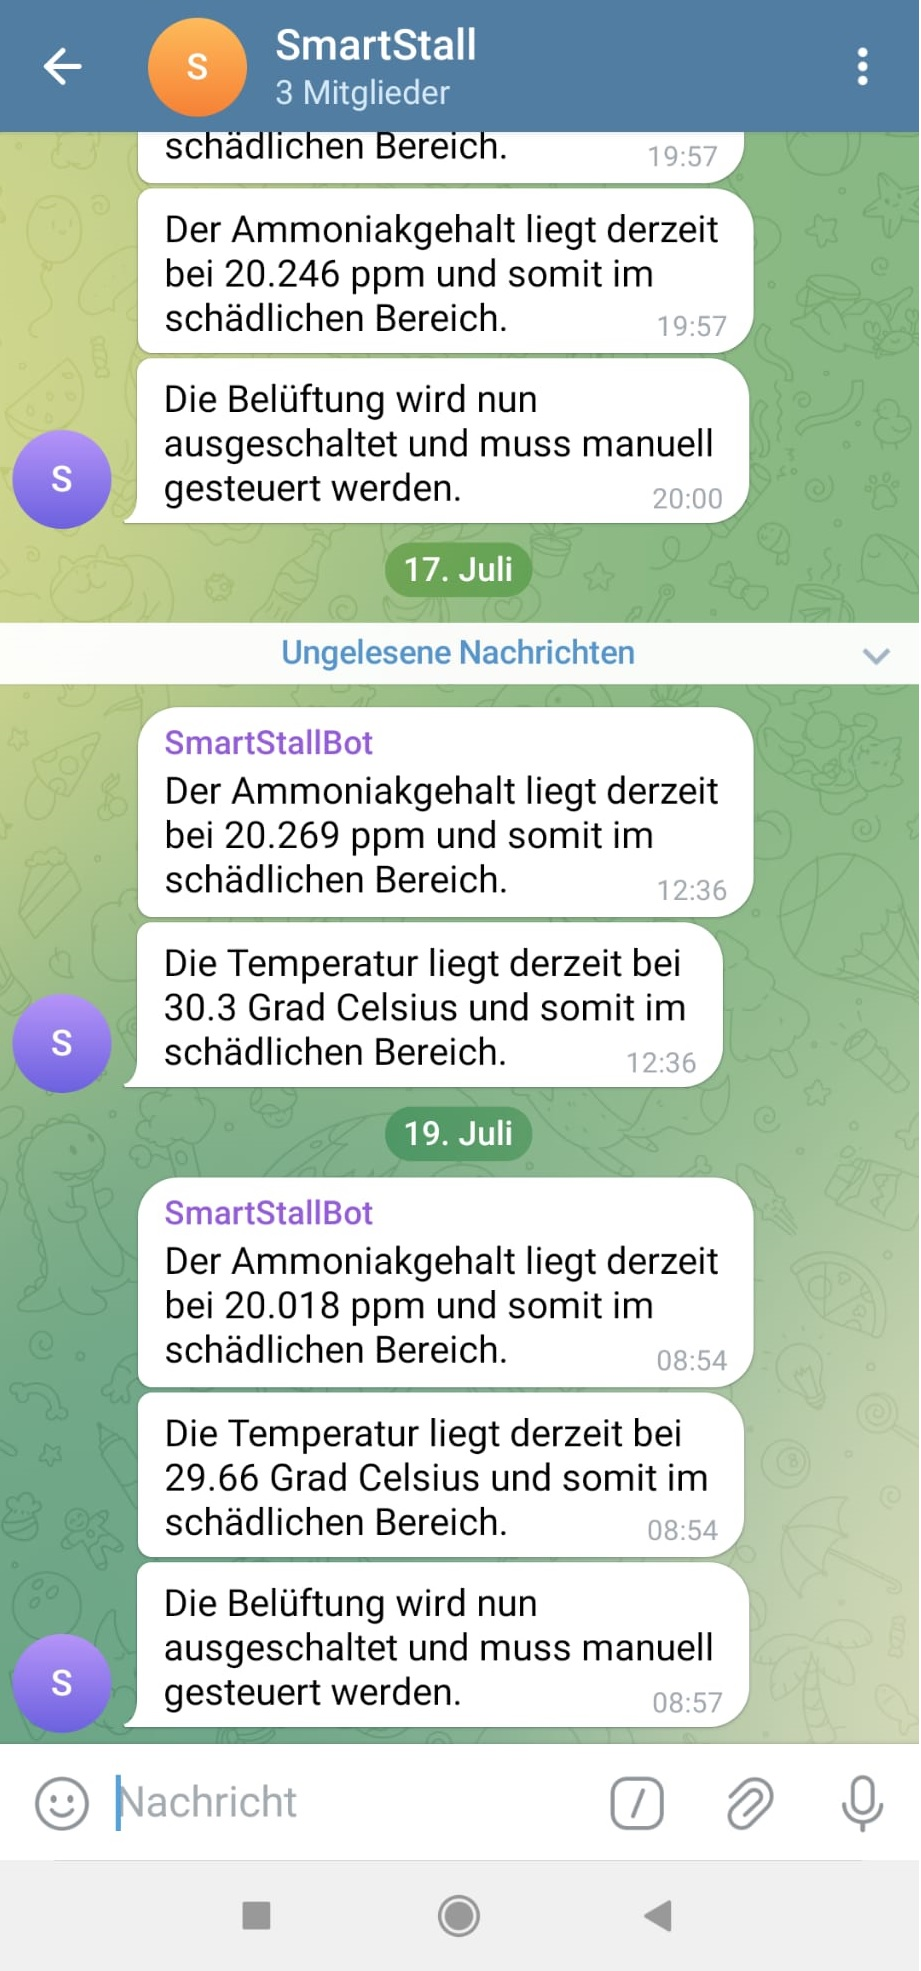
\includegraphics[width=60mm]{fig/uiTelegram.jpg}
	\caption{Beispielnachrichten der Telegramgruppe}
	\label{telegram}
\end{figure}
\subsection{Login-Seite}
Die Login-Seite besteht aus einem Formular, in das der Benutzername und das zugehörige Passwort eingegeben werden müssen. Bei fehlerhaften Eingaben wird ein Popup-Fenster angezeigt, das den Benutzer auffordert, die Daten erneut einzugeben. Bei korrekten Anmeldedaten erfolgt eine Weiterleitung zur Hauptseite.
Das Formular für die Benutzereingaben wird mithilfe des Frameworks Bootstrap erstellt, um die Implementierung der Login-Seite zu vereinfachen. Nach dem Ausfüllen der Eingabefelder und dem Klicken auf \textit{Anmelden} werden die Daten über einen AJAX-Aufruf an den Controller gesendet, wo sie überprüft werden.
\subsection{Benutzeroberfläche}
\label{ui}
Oben auf der Seite befindet sich der Titel "SmartStall", der den Namen des Projekts kennzeichnet. Direkt darunter sind zwei Schalter platziert: Mit dem Schalter "Benachrichtigung" können Benachrichtigungen aktiviert oder deaktiviert werden. Bei Aktivierung werden Benachrichtigungen über Telegram gesendet, wenn die Messwerte bestimmte Grenzwerte überschreiten. Der Schalter "Belüftung" dient dazu, die automatische Belüftung ein- oder auszuschalten. Wenn dieser Schalter aktiviert ist, schaltet sich die Belüftung automatisch ein, sobald die Messwerte über die festgelegten Grenzwerte steigen. \\
Die Webanwendung umfasst drei Hauptsektionen zur Überwachung der Luftqualität: Ammoniak, Luftfeuchtigkeit und Temperatur. Jede dieser Sektionen enthält ein interaktives Diagramm, das die Messwerte über einen Tages- oder Wochenverlauf anzeigt, je nach gewählter Ansicht und alle 3 Minuten aktualisiert wird. Die y-Achse der Diagramme zeigen die gemessenen Werte wie die Ammoniakkonzentration in ppm (parts per million), die Luftfeuchtigkeit in Prozent oder die Temperatur in Grad Celsius. Eine schwarze Linie stellt die aktuellen Messwerte dar, während eine rote Linie die festgelegten Grenzwerte anzeigt. \\
Neben jedem Diagramm wird der aktuelle Messwert groß und deutlich angezeigt. Dieser Wert ist grün hinterlegt, wenn er unterhalb der festgelegten Grenzwerte liegt, und rot hinterlegt, wenn er die Grenzwerte überschreitet. Dies ermöglicht den Benutzern, die aktuellen Bedingungen im Stall schnell zu erkennen. Die strukturierte Gestaltung des Interface stellt sicher, dass alle wichtigen Informationen auf einen Blick verfügbar sind und einfach verwaltet werden können. Das Userinterface kann dem Anhang \ref{sec:uiPCAnhang} für den PC und der Abbildung \ref{uiHandy} für ein Smartphone entnommen werden entnommen werden. 
\begin{figure}[h]
	\centering
	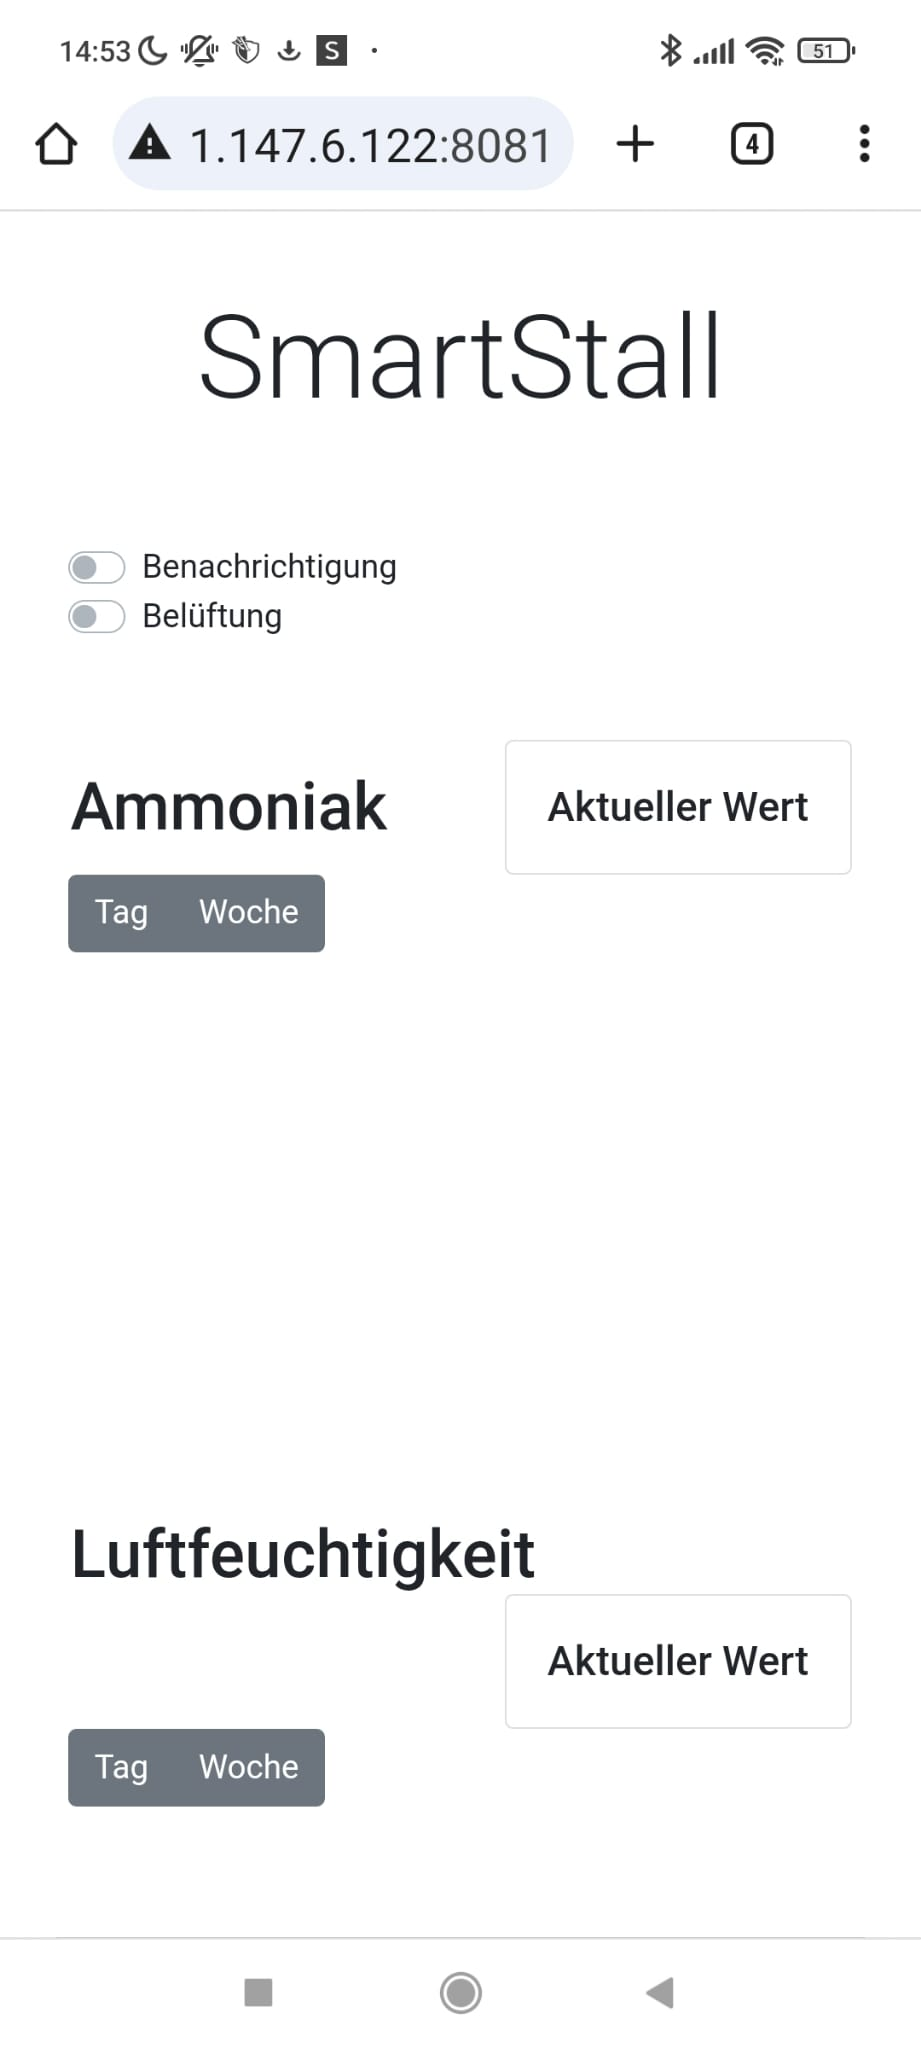
\includegraphics[width=42mm]{fig/uiHandy.jpg}
	\caption{Userinterface auf dem Smartphone}
	\label{uiHandy}
\end{figure}
\newpage
Auf einem Smartphone kann die Webanwendung zusätzlich durch die Einstellung "Zum Startbildschirm hinzufügen" im Browser an den Bildschirm angeheftet werden. Das für SmartStall entworfene Icon enthält die Initialien "ST" sowie Abbildungen eines Schweins, einer Kuh und eines Huhns. Unter diesem Logo, das in Abbildung \ref{stApp} zu sehen ist, wird die Webanwendung auf dem Smartphone sichtbar und kann wie eine App verwendet werden.
\begin{figure}[h]
	\centering
	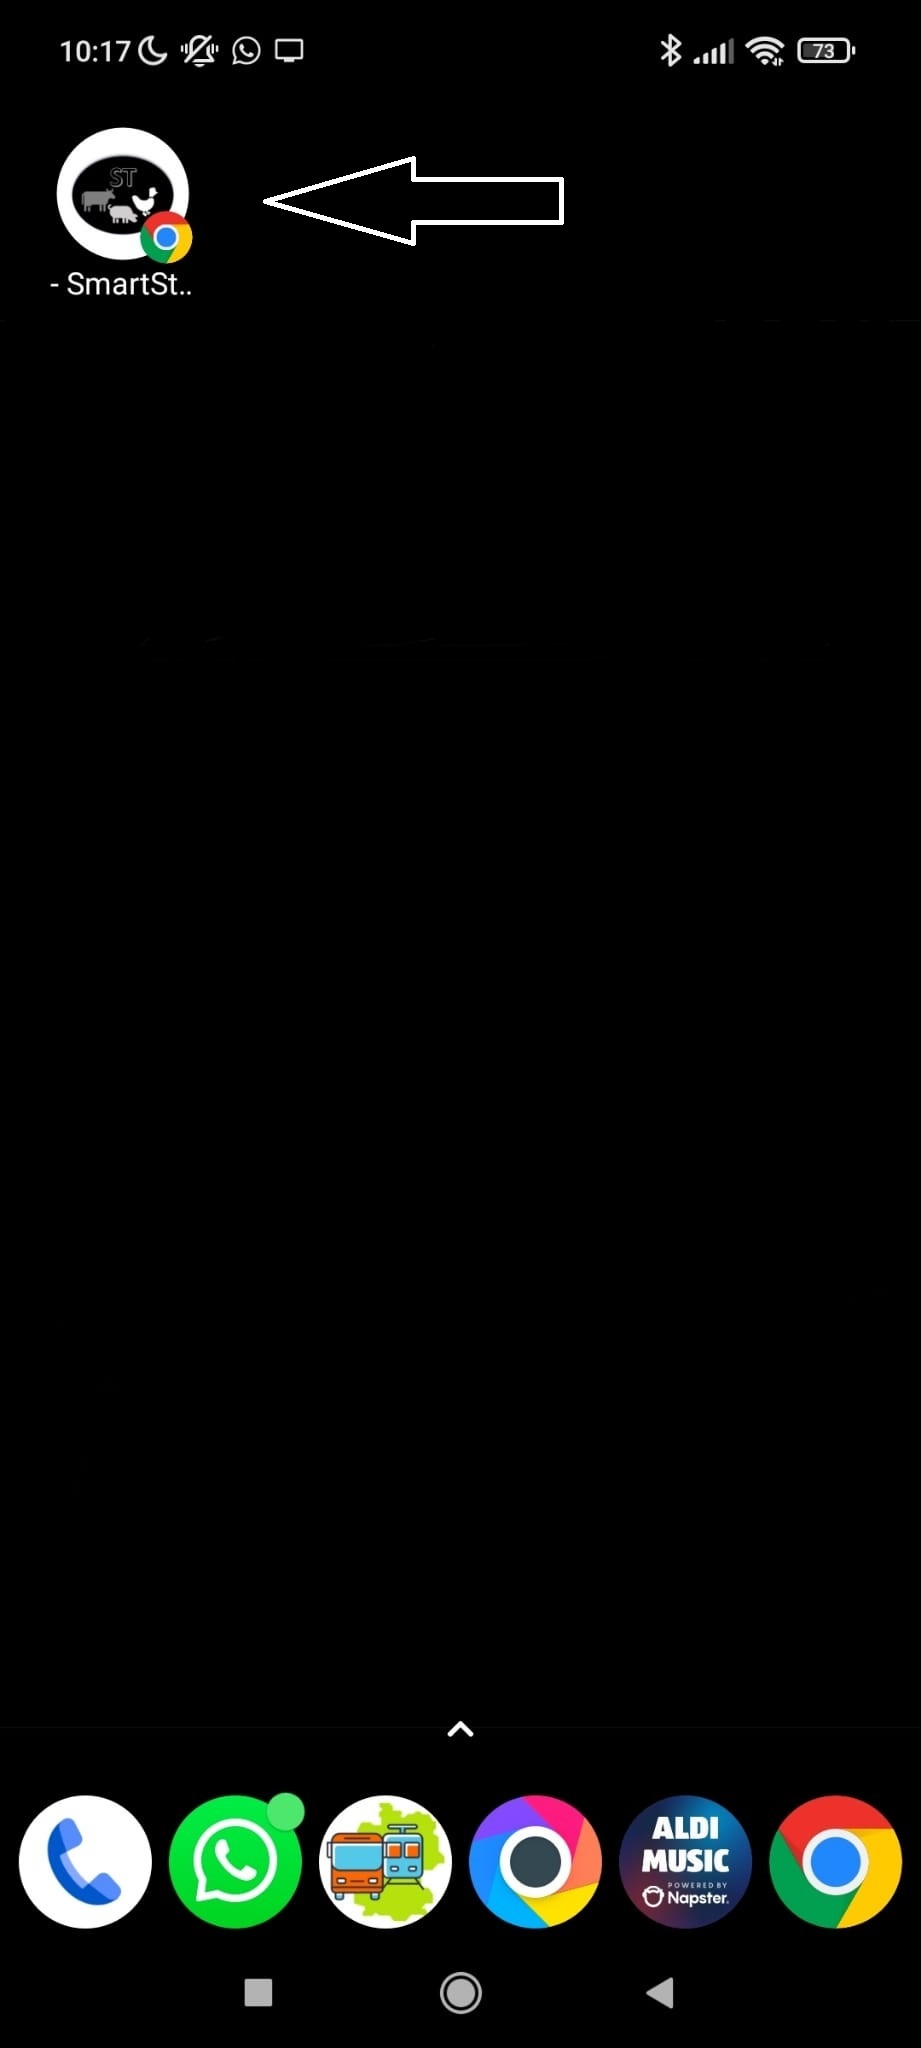
\includegraphics[width=42mm]{fig/stApp.jpg}
	\caption{Speichern der Webanwendung auf dem Startbildschirm des Smartphones, wodurch diese als App bedienbar ist}
	\label{stApp}
\end{figure}

\subsection{Ansteuerung der Steckdose}
Um die Belüftung zu steuern, ist es notwendig, eine WLAN-Steckdose zu integrieren, die mittels einer POST-Anfrage ein- oder ausgeschaltet werden kann. Zunächst muss die Steckdose mit dem WLAN verbunden werden. Dies erfolgt, indem die Steckdose an eine Stromquelle angeschlossen wird. Daraufhin kann man sich mit einem WLAN-fähigen Endgerät mit der Steckdose verbinden und diese über dessen Benutzeroberfläche konfigurieren. Hierbei lässt sich einstellen, mit welchem WLAN-Router die Steckdose verbunden werden soll, indem der Name des WLANs des Landwirtes und das zugehörige Passwort eingegeben wird. Nach einem Neustart verbindet sich die WLAN-Steckdose mit dem angegebenen Netzwerk. \\
Ist die Steckdose erfolgreich eingerichtet, kann sie entweder über das User Interface oder einen POST-Befehl im lokalen Netzwerk gesteuert werden. Beispielsweise kann folgende URL verwendet werden, um die Steckdose einzuschalten: \textit{http://localhost/cm?cmnd=Power\%20On}. Diese URL funktioniert jedoch nur innerhalb des eigenen Netzwerks \cite{delock}. Um die Steckdose auch außerhalb des eigenen Netzwerks steuern zu können, sind zusätzliche Schritte erforderlich:
\subsubsection{Dyndns}
Einerseits muss ein sogenanntes DynDNS eingerichtet werden. DynDNS (Dynamic Domain Name System) ermöglicht den Zugriff auf das Heimnetzwerk über das Internet, indem eine dynamische IP-Adresse in eine statische Domain umgewandelt wird. Dies erfolgt durch Registrierung bei einem DynDNS-Anbieter (in diesem Projekt der Anbieter dyndnsfree) und die Konfiguration des Dienstes auf dem Router, um eine Domain zu erstellen, die auf die dynamische IP-Adresse verweist \cite{dyndns}.
\subsubsection{Portfreigabe}
Für die Portfreigabe muss man sich in die Benutzeroberfläche des Routers einloggen und die Einstellungen für die Portweiterleitung suchen. Hier wird eine Regel hinzugefügt, die den Port (in diesem Projekt der Port 80), über den die WLAN-Steckdose kommuniziert, an deren lokale IP-Adresse weiterleitet \cite{portfreigabe}. Durch diese Konfiguration wird die Steckdose über das Internet erreichbar und kann entsprechend gesteuert werden. Die URL zur Steuerung sieht nun folgendermaßen aus: \textit{http://wlansteckdose.dnsuser.de/cm?cmnd=Power\%20On}

\section{Test des gesamten Systemaufbaus}
\subsection{Lokaler Test}
Für den Test der lokalen Webanwendung musste zunächst ein Python-Skript erstellt werden, das regelmäßig Daten in die Testdatenbank schreibt. Da der Raspberry Pi die Sensordaten nur in die produktive Datenbank schreibt, die sich auf dem Server befindet und somit für die lokale Anwendung nicht zugänglich ist, musste das Senden der Sensordaten simuliert werden. Das Python-Skript verbindet sich mit der Testdatenbank und schreibt minütlich Daten für Ammoniak, Temperatur und Luftfeuchtigkeit, jeweils mit Zeitstempel, in die Datenbank. Dabei wurden Grenzen definiert, innerhalb derer sich die Daten befinden dürfen: Ammoniak zwischen 15 und 25, Temperatur zwischen 20 und 28, und Luftfeuchtigkeit zwischen 50 und 65. \\
Die Webanwendung wurde lokal getestet. Dabei wurden beide Schalter auf der Hauptseite der Benutzeroberfläche (Benachrichtigung und Belüftung) eingeschaltet und überprüft, ob diese gemäß der eingebauten Logik arbeiten und die Diagramme mit den entsprechenden Werten aktualisiert werden. Anschließend wurde der Schalter für die Belüftung ausgeschaltet und überprüft, ob eine Nachricht gesendet wird, die darüber informiert, dass die Belüftung ausgeschaltet ist und manuell gesteuert werden muss. Der lokale Test war erfolgreich. \\
\subsection{Produktiver Test}
Der Test für die produktive Webanwendung verlief ähnlich. Zunächst wurde geprüft, ob der Raspberry Pi die Sensordaten mit dem korrekten Zeitstempel an die Webanwendung schickt. Hierfür wurde die Log-Datei verwendet, welche bereits in Kapitel \ref{chapter:datenuebertragung}
beschrieben wurde. \\
Anschließend wurde überprüft, ob die Daten korrekt in der Webanwendung visualisiert werden. Wie im lokalen Test wurden die Schalter für Benachrichtigung und Belüftung eingeschaltet. Der RaspberryPi wurde von einem Dachgeschosszimmer in den Keller umgestellt. Dementsprechend fiel die Temperatur und stieg die Luftfeuchtigkeit, wie in Anhang \ref{sec:testDiagramm} zu sehen ist. \\
Die Temperaturwerte lagen vor der Verlagerung über der festgelegten Grenze von 25. Die Benachrichtigung wurde korrekt gesendet und die WLAN-Steckdose eingeschaltet. Anschließend wurde der Schalter für die Belüftung ausgeschaltet und überprüft, ob eine Nachricht gesendet wird, die darüber informiert, dass die Belüftung ausgeschaltet ist und manuell gesteuert werden muss. Nach der Verlagerung in den Keller sanken und alle Werte unter die Grenzen. Dementsprechend schaltete sich die WLAN-Steckdose automatisch aus. Der produktive Test war ebenfalls erfolgreich.

\section{Zusammenfassung}
Das Projekt Smartstall behandelt die Schnittstellen und Datenübertragung von Endgeräten sowie deren Anbindung an die Cloud nach dem Internet of Things Konzept. Das Projekts erfasst verschiedene Sensordaten zur Überwachung der Luftqualität in einem Stall. Die erfassten Daten werden über einen Raspberry Pi an eine eigens entwickelte Webanwendung gesendet, sodass der Anwender die Möglichkeit hat, die Daten über eine benutzerfreundliche Oberfläche anzuzeigen und zu analysieren. \\
Bei Überschreitung bestimmter, festgelegter Schwellwerte wie Temperatur, Luftfeuchtigkeit oder Ammoniakgehalt, wird der Anwender per Push-Benachrichtigung auf seinem Smartphone informiert. Zusätzlich wird die Belüftung bei Bedarf automatisch ein- und ausgeschaltet. Dies wird wie beschrieben durch die Steuerung der WLAN-Steckdose umgesetzt. \\
Die Anforderungen an das Projekt wurden in Rücksprache mit zwei verschiedenen landwirtschaftlichen Betrieben angepasst, da die Betriebe  vor allem Wert auf eine einfache Anwendung und die Möglichkeit, die automatisierte Steuerung der Belüftung und die Push-Benachrichtigungen ein- und ausschalten zu können, legten. \\
Zur Erfassung der Luftqualitätsdaten kommt ein Raspberry Pi zum Einsatz, welcher mit den beschriebenen Sensoren ausgestattet ist. Die erfassten Daten werden in eine Datenbank geschrieben und anschließend von der Webanwendung ausgelesen und visualisiert. Die Webseite kann auch außerhalb des Netzwerks des Landwirts genutzt werden, um die Belüftung und Push-Benachrichtigungen zu steuern. Smartstall bietet somit eine kostengünstige Alternative zur automatisierten Steuerung und Kontrolle der Luftqualitätsdaten in einem Stall. \\
\newpage
\section{Ausblick}
Um das ProjektSmartStall in Zukunft weiter auszubauen, gibt es verschiedene Möglichkeiten. Ein Vorteil wäre es, die Luftqualität nicht nur an einem Punkt, sondern an mehreren Stellen im Stall zu messen, da die Luftqualität in einem großen Stall an verschiedenen Punkten unterschiedlich sein kann. Mehrere Sensoren könnten im Stall installiert werden, um einen detaillierteren Einblick in die Luftqualität zu erhalten. Entsprechend könnte auch die Belüftung nur in bestimmten Bereichen des Stalls aktiviert werden. Falls mehrere Sensoren verbaut werden, könnte das Userinterface umgestaltet werden, sodass der Landwirt sehen kann, an welchen Punkten im Stall die Luftqualität schlecht ist. \\
Ein weiterer Aspekt zur Verbesserung des Projekts ist der Ausbau der Datenbank. Wenn SmartStall von mehreren Landwirten genutzt wird, ist es sinnvoll, Nutzerdaten in der Datenbank zu hinterlegen, inklusive Logindaten. Für jeden Nutzer könnten auch individuelle Parameter wie die Grenzwerte hinterlegt werden. Dadurch besteht die Möglichkeit, ein individuelles Dashboard basierend auf den Daten aus der Datenbank zu erstellen. \\
Zwei weitere Punkte betreffen den Ausbau der Funktionen, die dem Landwirt in der Webanwendung zur Verfügung stehen. Zum einen könnte eine Einstellungsseite hinzugefügt werden, auf der der Landwirt selbst die Grenzwerte für verschiedene Luftqualitätsdaten festlegen kann. Zum anderen wäre es möglich, dass der Landwirt auf Benachrichtigungen über eine Schwellwertüberschreitung in Telegram antworten und auf diesem Weg die Belüftung anschalten kann. Dies könnte jedoch dazu führen, dass einige Landwirte sich überfordert fühlen, aufgrund von mangelndem technischen Verständnis. \\
Insgesamt bietet SmartStall viel Potenzial für den weiteren Ausbau des Projekts.

\newpage
\begin{thebibliography}{00}

\bibitem{ammoniak}
Bayerischer Rundfunk, "Ammoniak - giftiger Grundstoff für Sprengstoff und Dünger", Online. Verfügbar unter: https://www.br.de/nachrichten/wissen/ammoniak-gas-reizendes-kaeltemittel-fuer-augen-und-atemwege,RLvCroD. [Zugriffsdatum: 18. Juli 2024].

\bibitem{luftfeuchtigkeit}
Stuttgarter Zeitung Verlagsgesellschaft mbH, "Ab welcher Luftfeuchtigkeit entsteht Schimmel?", Online. Verfügbar unter: https://www.stuttgarter-zeitung.de/inhalt.ab-welcher-luftfeuchtigkeit-schimmel-mhsd.54e71b67-c3b7-4820-a80a-abcb4061c18b.html. [Zugriffsdatum: 18. Juli 2024].

\bibitem{temperatur}
DLG e. V., "Hitzestress im Stall? Erkennen und Maßnahmen", Online. Verfügbar unter: https://www.fokus-tierwohl.de/de/rind/fachinformationen-milchvieh/hitzestress-bei-milchkuehen. [Zugriffsdatum: 18. Juli 2024].

\bibitem{raspy}
Raspberry Pi Foundation, "Raspberry Pi", Online. Verfügbar unter: https://www.raspberrypi.com. [Zugriffsdatum: 20. Juli 2024].

\bibitem{bme}
Joy-It, "BME680", Online. Verfügbar unter: https://joy-it.net/de/products/SEN-BME680. [Zugriffsdatum: 20. Juli 2024].

\bibitem{bmeDataSheet}
https://www.bosch-sensortec.com/products/environmental-sensors/gas-sensors/bme680/ [Zugriffsdatum: 05. August 2024].

\bibitem{mqDataSheet}
https://www.winsen-sensor.com/d/files/semiconductor/mq137.pdf [Zugriffsdatum: 05. August 2024].

\bibitem{bmeAbbildungen}
https://www.laub-home.de/wiki/Raspberry\_Pi\_BME680\_Gas\_Sensor [Zugriffsdatum: 20. Juli 2024].

\bibitem{bme_anschluss}
Laub-Home Wiki, "Raspberry Pi BME680 Gas Sensor", Online. Verfügbar unter: https://www.laub-home.de/wiki/Raspberry\_Pi\_BME680\_Gas\_Sensor. [[Zugriffsdatum: 20. Juli 2024].

\bibitem{i2cDoc}
https://www.nxp.com/docs/en/user-guide/UM10204.pdf [Zugriffsdatum: 05. August 2024].

\bibitem{crontab}
https://help.ubuntu.com/community/CronHowto [Zugriffsdatum: 05. August 2024].

\bibitem{dotNET}
Microsoft Corporation, ".NET-Dokumentation", Online. Verfügbar unter: https://learn.microsoft.com/de-de/dotnet/. [Zugriffsdatum: 18. Juli 2024].

\bibitem{csharp}
Microsoft Corporation, "C\#-Dokumentation", Online. Verfügbar unter: https://learn.microsoft.com/de-de/dotnet/csharp/tour-of-csharp/. [Zugriffsdatum: 18. Juli 2024].

\bibitem{mvc}
Heise Medien GmbH \& Co. KG, "Patterns in der Softwarearchitektur: Model-View-Controller ", Online. Verfügbar unter: https://www.heise.de/blog/Patterns-in-der-Softwarearchitektur-Model-View-Controller-8956787.html. [Zugriffsdatum: 18. Juli 2024].

\bibitem{bootstrap}
JavaScript Bootstrap, "Get started with Bootstrap", Online. Verfügbar unter: https://getbootstrap.com/docs/5.3/getting-started/introduction/. [Zugriffsdatum: 05. Juli 2024].

\bibitem{grafana}
Grafana Labs, "Grafana documentation", Online. Verfügbar unter: https://grafana.com/docs/grafana/latest/. [Zugriffsdatum: 05. Juli 2024].

\bibitem{chart.js}
Chart.js, "Line Chart", Online. Verfügbar unter: https://www.chartjs.org/docs/latest/charts/line.html. [Zugriffsdatum: 05. Juli 2024].

\bibitem{telegram}
Telegram Foundation, "Telegram APIs", Online. Verfügbar unter: https://core.telegram.org/. [Zugriffsdatum: 05. Juli 2024].

\bibitem{delock}
Delock, "Wlan Power Socket Switch", Online. Verfügbar unter: https://www.delock.de/files/71415.download. [Zugriffsdatum: 05. Juli 2024].

\bibitem{dyndns}
AVM Foundation, "Dynamic DNS in FRITZ!Box einrichten", Online. Verfügbar unter: https://avm.de/service/wissensdatenbank/dok/FRITZ-Box-7590/30\_Dynamic-DNS-in-FRITZ-Box-einrichten/. [Zugriffsdatum: 05. Juli 2024].

\bibitem{portfreigabe}
AVM Foundation, "Portfreigabe in FRITZ!Box einrichten", Online. Verfügbar unter: https://avm.de/service/wissensdatenbank/dok/FRITZ-Box-7490/34\_Portfreigaben-in-FRITZ-Box-einrichten/. [Zugriffsdatum: 05. Juli 2024].

\end{thebibliography}

\clearpage
\begin{appendices}
	\section{Aufbau und Zusammenspiel der Komponenten}
	\label{sec:AufbauAnhang}
	\begin{figure}[h]
		\centering
		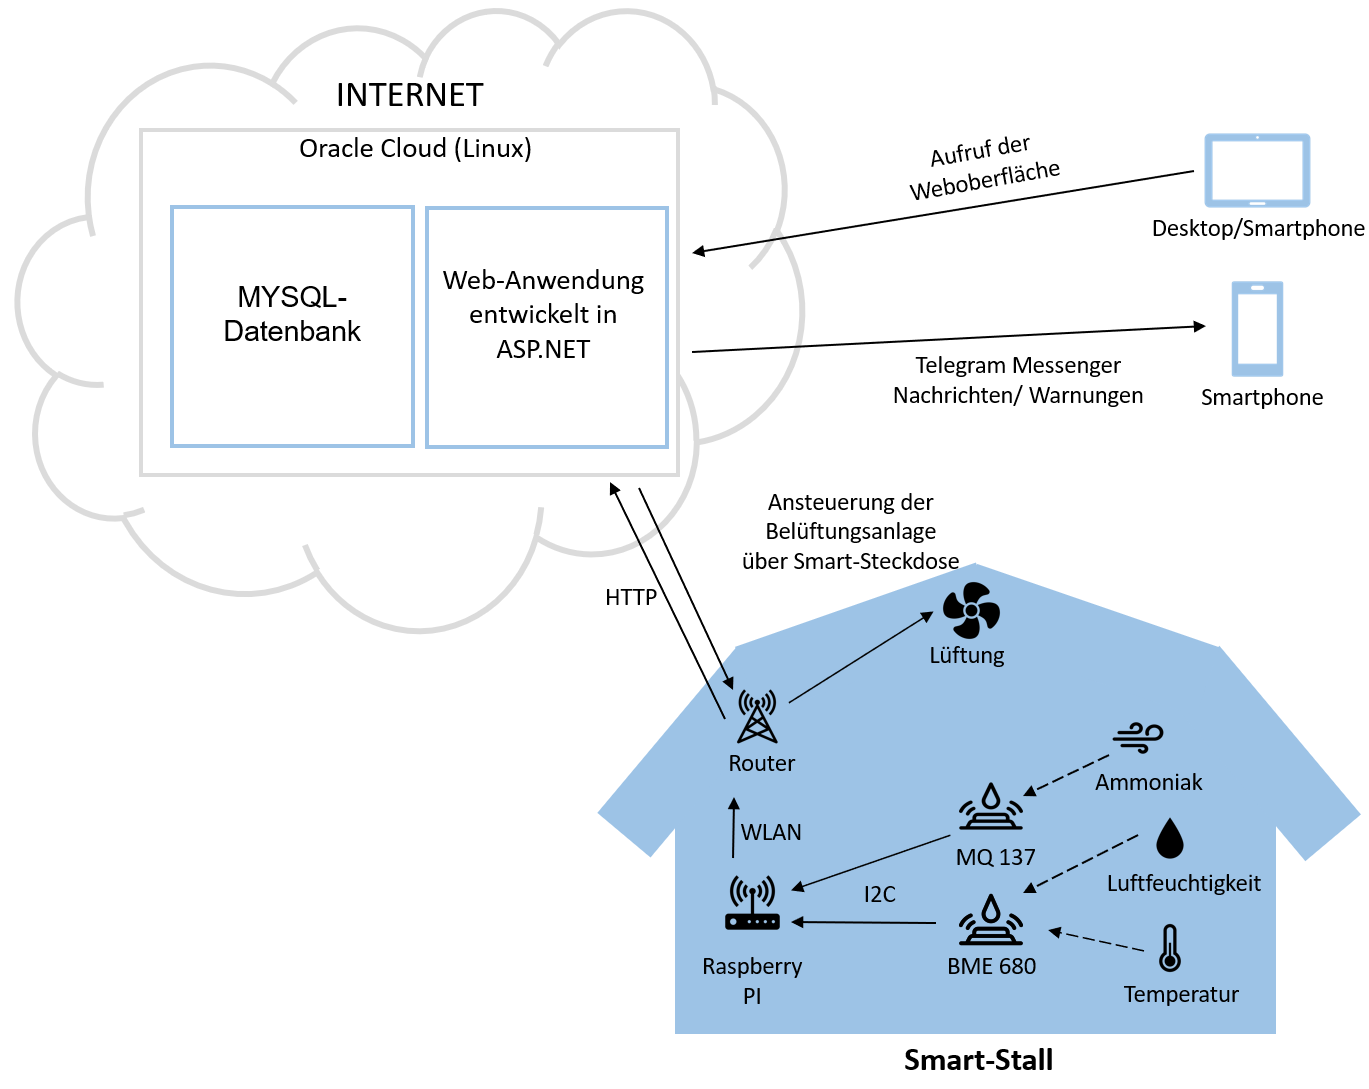
\includegraphics[width=0.99\textwidth]{fig/Projektaufbau.png}
	\end{figure}
	
\clearpage
\section{HTML-Code für Digrammabschnitt}
\label{sec:htmlCodeDiagrammAnhang}
\begin{figure}[h]
    \centering
    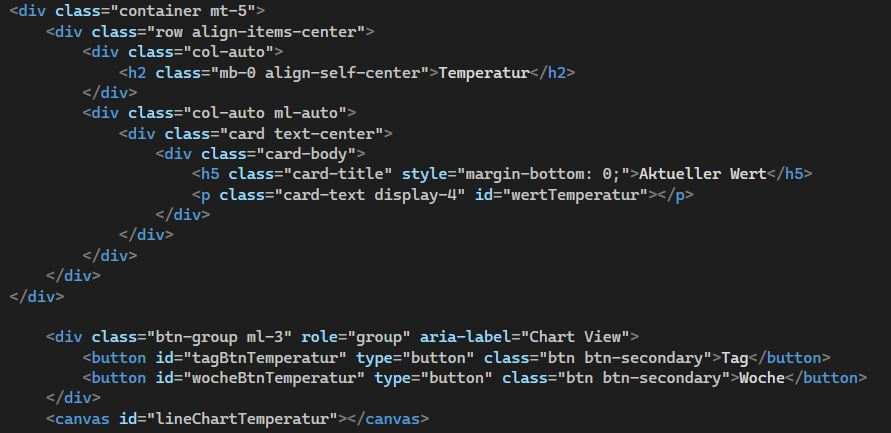
\includegraphics[width=0.99\textwidth]{fig/htmlcode.JPG}
\end{figure}

\clearpage
\section{Userinterface PC}
\label{sec:uiPCAnhang}
\begin{figure}[h]
    \centering
    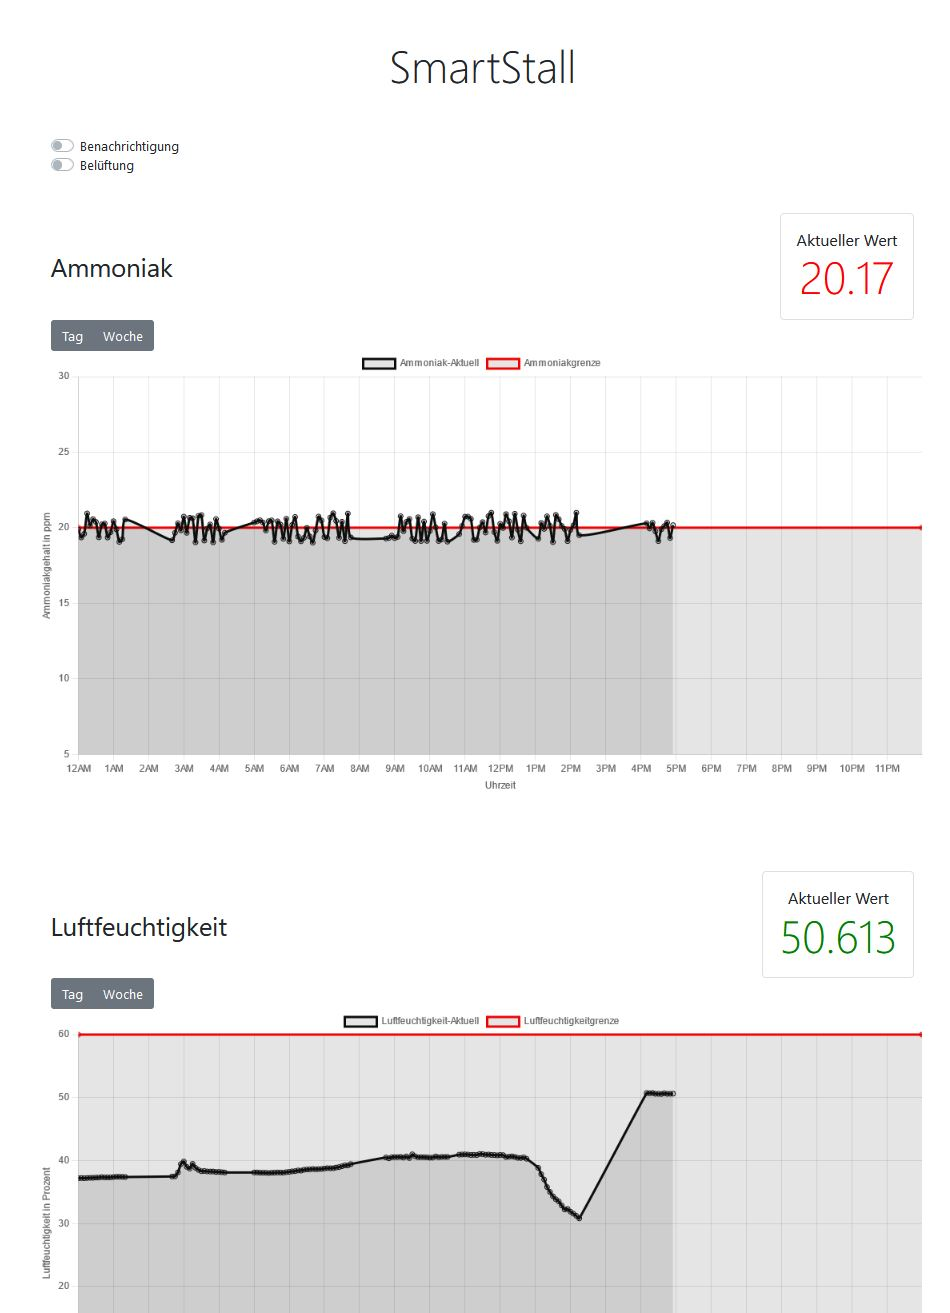
\includegraphics[width=0.8\textwidth]{fig/uiPC.jpg}
\end{figure}

\clearpage
\section{AJAX-Aufruf, um Sensordaten asynchron zu laden}
\label{sec:ajaxAnhang}
\begin{figure}[h]
    \centering
    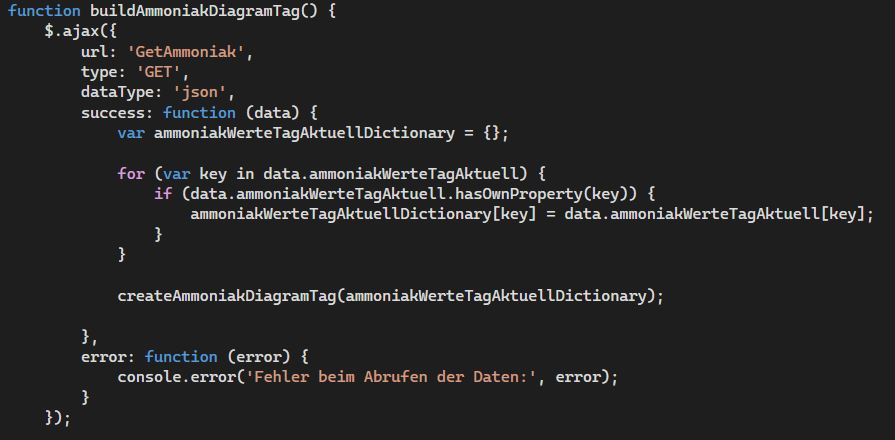
\includegraphics[width=0.99\textwidth]{fig/ajax.JPG}
\end{figure}

\clearpage
\section{Java-Scriptcode zum Aufbau eines Diagramms}
\label{sec:jsdiagrammanhang}
\begin{figure}[h]
    \centering
    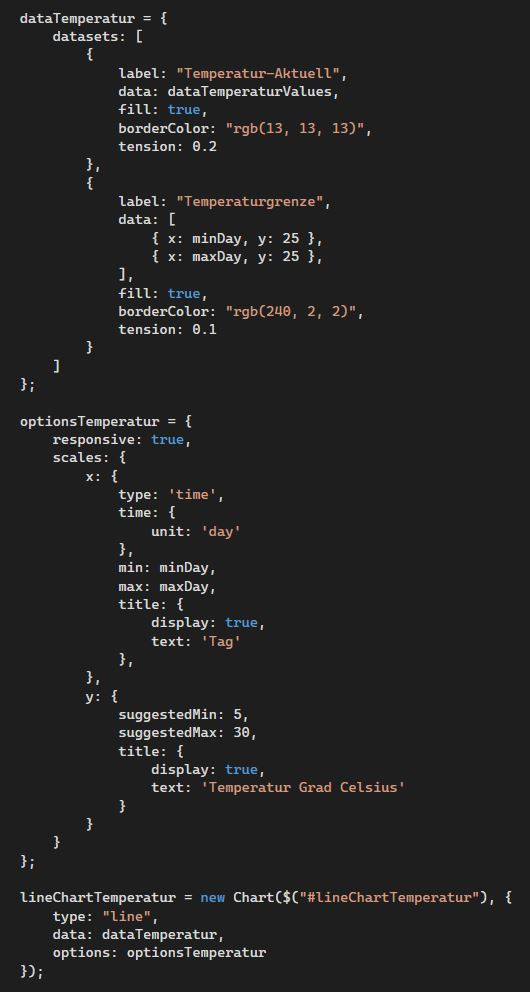
\includegraphics[width=0.60\textwidth]{fig/diagrammCode.JPG}
\end{figure}

\clearpage
\section{Produktiver Test}
\label{sec:testDiagramm}
\begin{figure}[h]
    \centering
    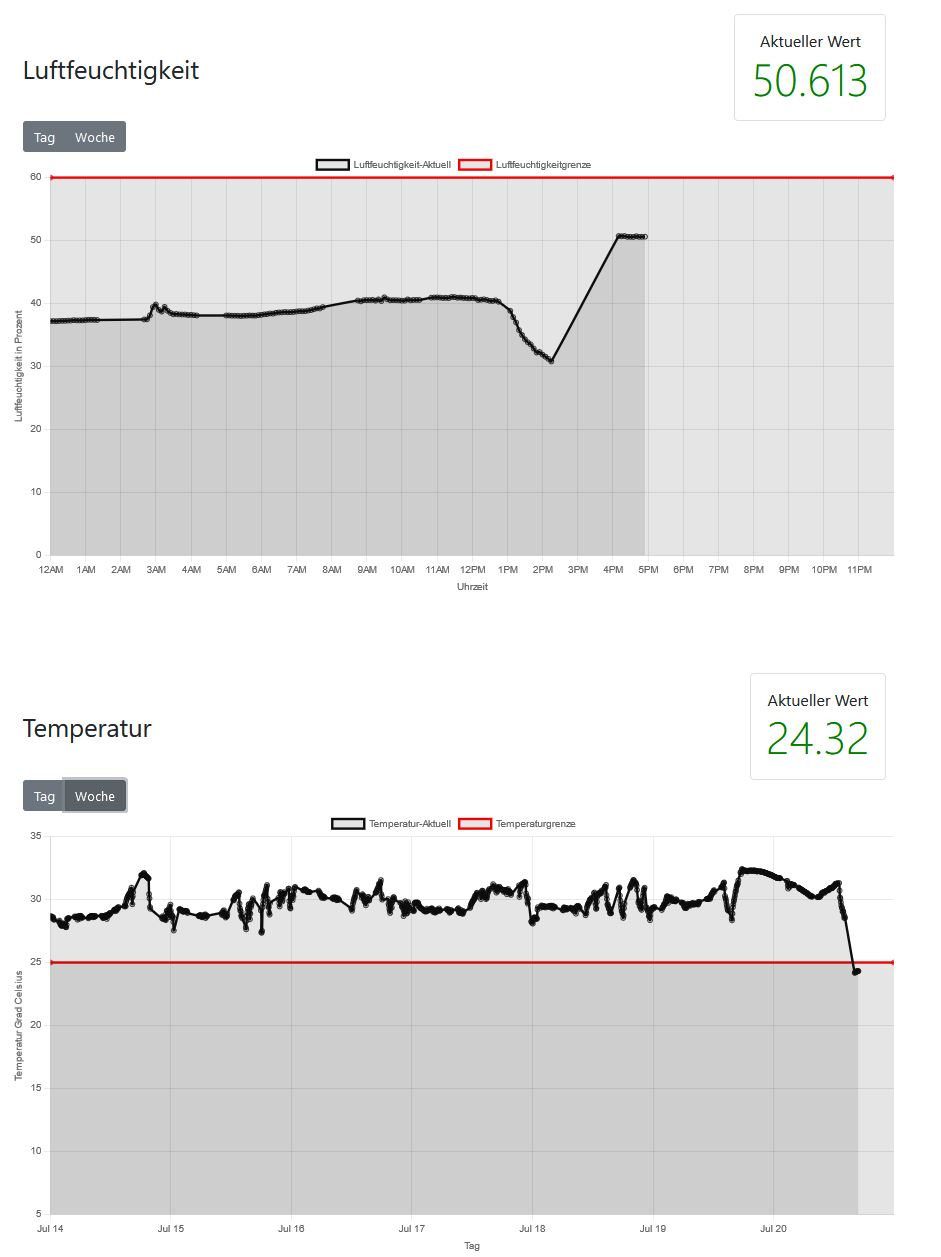
\includegraphics[width=0.8\textwidth]{fig/test.JPG}
\end{figure}

\end{appendices}

\end{document}
